\chapter{Scaling with error rate} \label{ch:global}

\graphicspath{{\dir/}}

The trie index from \cref{ch:trie} enabled sublinear scaling with the reference
size, and the seed heuristic from \cref{ch:seed} additionally enabled long
queries to be aligned. Nevertheless, when there are too many errors (more than
1\% for long sequences), the seed heuristic may not be able to compensate for
all of them, and the search has to start exporing in width (similar to
Dijkstra).

In this chapter we consider the more basic problem of global alignment between
two sequences and demonstrate how to squeeze out more information from each seed
by aligning it inexactly (with up to 1 edit), as well as from the connection
between the seeds by chaining them in order in both sequences. As a result, we
reach near-linear scaling to long sequence for error rates as high as $15\%$ and
orders of magnitude of speedup compared to other optimal aligners for $5\%$
error rate. 

% This text will be sanitized and placed into lqa-output/abstract.txt
%
Motivation and approach: the trie index works for scaling sublinerly with the
reference size but each error in the query triggers deeper exploration of the
trie so the runtime grows exponentially. Lets inform the \A algorithm using
information from the whole query length while keeping the trie. This way we
could avoid the deep trie exploration and scale to long queries (as far as the
error rate is not too high).

We present a novel \A \emph{\seedh} that enables fast and optimal
sequence-to-graph alignment, guaranteed to minimize the edit distance of the
alignment assuming non-negative edit costs.

We phrase optimal alignment as a shortest path problem and solve it by
instantiating the \A~algorithm with our \seedh. The \seedh first extracts
non-overlapping substrings (\emph{seeds}) from the read, finds exact seed
\emph{matches} in the reference, marks preceding reference positions by
\emph{crumbs}, and uses the crumbs to direct the \A search. The key idea is to
punish paths for the absence of foreseeable seed matches. We prove admissibility
of the \seedh, thus guaranteeing alignment optimality.

\qquad Our implementation extends the free and open source aligner and
demonstrates that the \seedh outperforms all state-of-the-art optimal aligners
including \graphaligner, \vargas, \pasgal, and the \prefixh previously employed
by \astarix. Specifically, we achieve a consistent speedup of >60$\times$ on
both short Illumina reads and long HiFi reads (up to 25kbp), on both the
\textit{E.~coli} linear reference genome (1Mbp) and the MHC variant graph
(5Mbp). Our speedup is enabled by the \seedh consistently skipping >99.99\% of
the table cells that optimal aligners based on dynamic programming
compute.\\

\astarix aligner and evaluations: \astarixurl\\

Genome graph, Optimal alignment, Semi-global alignment, Edit distance, Shortest
path, Long reads, \A algorithm, Seed heuristic
\section{Overview}

% General: aligning, edit distance
Alignment of reads to a reference genome is an essential and early step in most
bioinformatics pipelines. While linear references have been used traditionally,
an increasing interest is directed towards graph references capable of
representing biological variation~\citep{garrison_variation_2018}.
%
Specifically, a \emph{sequence-to-graph} alignment is a base-to-base
correspondence between a given read and a walk in the graph. As sequencing
errors and biological variation result in inexact read alignments, edit distance
is the most common metric that alignment algorithms optimize in order to find
the most probable read origin in the reference.

% We note that in contrast to linear references, reference graphs capture
% genomic variation and therefore enable more accurate
% alignments~\citep{garrison_variation_2018}.

\paragraph{Suboptimal alignment}
%
In the last decades, approximate and alignment-free methods satisfied the demand
for faster algorithms which process huge volumes of genetic
data~\citep{kucherov2019evolution}. 
%
\emph{Seed-and-extend} is arguably the most popular paradigm in read
alignment~\citep{altschul_basic_1990,langmead_fast_2012,li_fast_2009}. First,
substrings (called \emph{seeds} or \emph{kmers}) of the read are extracted, then
aligned to the reference, and finally prospective matching locations are
\emph{extended} on both sides to align the full read.

While such a heuristic may produce acceptable alignments in many cases, it
fundamentally does not provide quality guarantees, resulting in suboptimal
alignment accuracy.
%
In contrast, here we demonstrate that seeds can benefit optimal alignment as
well.

\paragraph{Key challenges in optimal alignment}
%
Finding optimal alignments is desirable but expensive in the worst case,
requiring $\Oh(Nm)$ time~\citep{equi2019complexity}, for graph size $N$ and read
length $m$.
%
Unfortunately, most optimal sequence-to-graph aligners rely on dynamic
programming (DP) and always reach this worst-case asymptotic runtime. Such
aligners include \vargas~\citep{darby2020vargas},
\pasgal~\citep{jain_accelerating_2019},
\graphaligner~\citep{rautiainen_bitparallel_2019},
\hga~\citep{feng2021accelerating}, and \vg~\citep{garrison_variation_2018},
which use bit-level optimizations and parallelization to increase their
throughput.

In contrast, we follow the promising direction of using a heuristic to avoid
worst-case runtime on realistic data. To this end, \astarix rephrases the task
of alignment as a shortest-path problem in an \emph{alignment graph} extended by
a \emph{trie index}, and solves it using the \A~algorithm instantiated with a
problem-specific \prefixh. Importantly, its choice of heuristic only affects
performance, not optimality.
%
Unlike DP-based algorithms, this \prefixh allows scaling sublinearly with the
reference size, substantially increasing performance on large genomes. However,
it can only efficiently align reads of limited length.

\paragraph{Contributions}
%
Here we address the key challenge of scaling to long HiFi reads, while
retaining the superior scaling of \astarix in the size of the reference graph.
%
To this end, we instantiate the \A algorithm with a novel \seedh, which
outperforms existing optimal aligners on both short and long HiFi reads.
%
Specifically, the \seedh utilizes information from the whole read to narrowly
direct the \A search by placing \emph{crumbs} on graph nodes which lead up to a
\emph{seed match}, \ie, an exact match of a substring of the read.

Overall, the contributions presented next include:
\begin{enumerate}
    \item A novel \A~\seedh that exploits information from the whole read to
    quickly align it to a general graphs reference.
    \item An optimality proof showing that the \seedh always finds an alignment
    with minimal edit distance.
	\item An implementation of the \seedh as part of the \astarix aligner.
    \item An extensive evaluation of our approach, showing that we align both
    short Illumina reads and long HiFi reads to both linear and graph references
    $\geq 60 \times$ faster than existing optimal aligners.
    \item A demonstration of superior empirical runtime scaling in the reference
    size $N$: $N^{0.46}$ on Illumina reads and $N^{0.11}$ on HiFi reads.
\end{enumerate}

\begin{figure}[t]
    \centering
	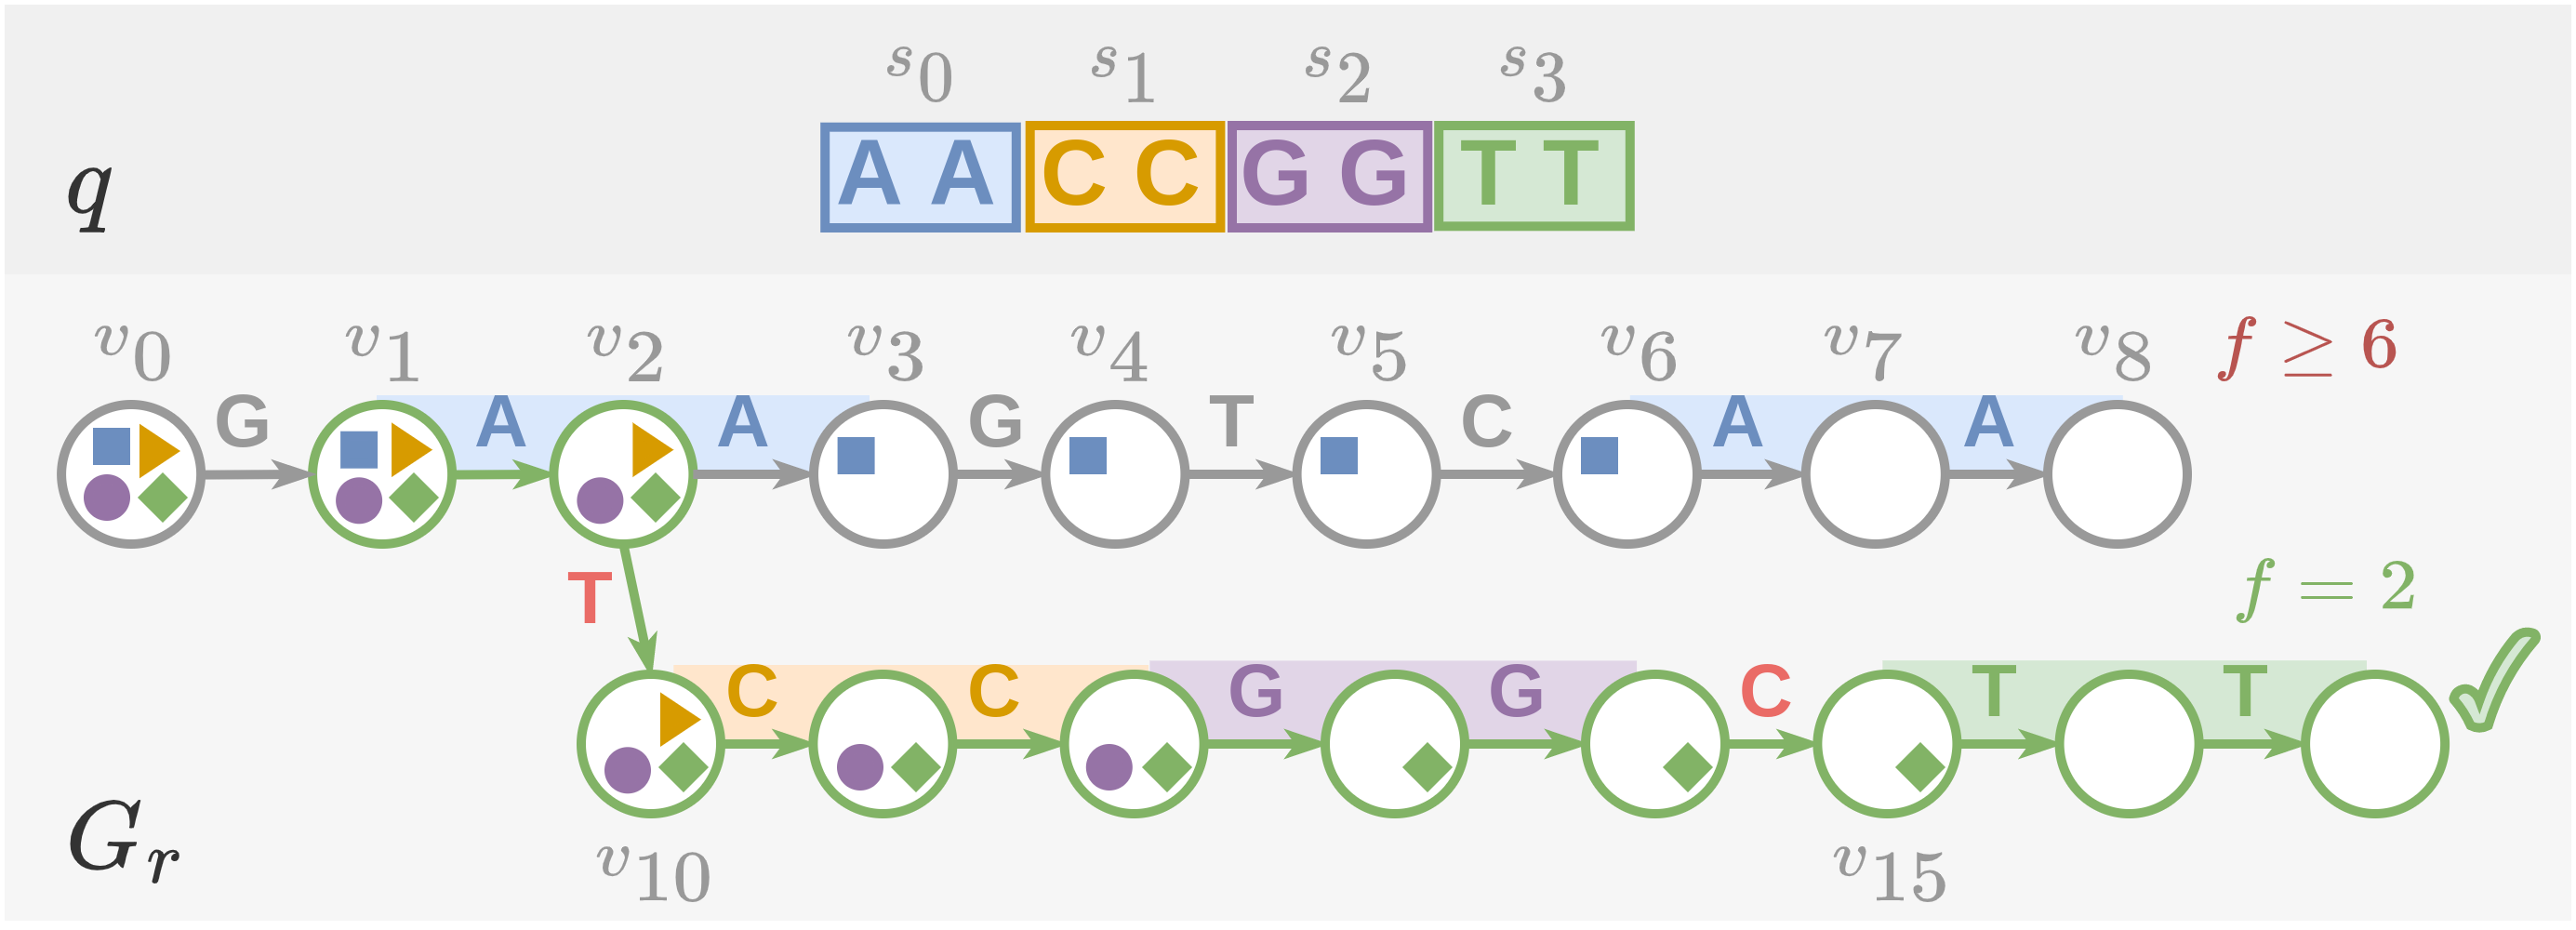
\includegraphics[width=0.6\linewidth]{figures/seed-heuristic-diagram.png}
	\caption{%
		A toy overview example using the \seedh to align a read $q$ to a
		reference graph $\RG$. The read is split into four colored seeds, where
		their corresponding crumbs are shown inside reference graph nodes as
		symbols with matching color. The optimal alignment is highlighted as a
		green path ending with a tick (\protect\greentick{}) and includes one
		substitution
		($\mathtt{\textcolor{dark-red}{T}{\rightarrow}\textcolor{dark-red}{A}}$)
		and one deletion ($\textcolor{dark-red}{\mathtt{C}}$).
		%
	}
\label{SEEDfig:overview}
\end{figure}

\paragraph{Intuition} \label{SEEDsec:overview}
% Task
\cref{SEEDfig:overview} showcases the \sh on an overview example. It shows a
read~$q$ to be aligned to a reference graph~$\RG$. Our goal is to find an
optimal alignment starting from an arbitrary node $v \in \RG$.
%
For simplicity of the exposition, we assume unit edit costs $\cedits =
(0,1,1,1)$, which we generalize in~\cref{SEEDsec:definition}.

\paragraph{Intuition}
The \A search requires us to provide a lower bound of the remaining path cost
from a state $\st{v}{i}$ to a target state. Clearly, to align the whole query,
each of the remaining seeds (\ie~at or after position $i$ in $q$) has to be
eventually aligned. The intuition underlying the \sh is to punish the state
for the absence of any foreseeable match of each remaining seed. Notice that the
order of the seeds is not directly taken into account.

In order to quickly check if a seed $s$ can lead to a match, we follow a
procedure similar to the one used by Hansel and Gretel who were placing
breadcrumbs to find their trail back home. Before aligning a query, we will
precompute all $\emph{crumbs}$ from all seeds so that not finding a crumb for
a seed $s$ on node $v$ indicates that seed $s$ could not be matched exactly
before the query is fully aligned continuing from $v$. This way, assuming that a
shortest path includes many seed matches, the crumbs will direct the \A search
along with it.

If a crumb from an expected seed is missing in node $v$, its corresponding seed
$s$ could not possibly be aligned exactly and this will incur the cost of at
least one substitution, insertion, or deletion. Assuming unit edit costs,
$h\st{v}{i}$ yields a lower bound on the cost for aligning $q[i{:}]$ starting
from $v$ by simply returning the number of missing expected crumbs in $v$.

\paragraph{Crumbs precomputation example}
%
\cref{SEEDfig:overview} shows four seeds as colored sections of length $2$ each, and
represents their corresponding crumbs as \bluecrumb{}, \yellowcrumb{},
\violetcrumb{} and \greencrumb{}, respectively. Four crumbs are expected if we
start at $v_2$, but \bluecrumb{} is missing, so $h\st{v_2}{0}=1$. Analogously,
if we reach $v_2$ after aligning one letter from the read, we expect 3 crumbs
(except \bluecrumb{}), and we find them all in $v_2$, so $h\st{v_2}{1}=0$.
%
To precompute the crumbs for each seed, we first find all positions in $\RG$
from which the seed aligns exactly. \cref{SEEDfig:overview} shows these exact
matches as colored sections of $\RG$. Then, from each match we traverse $\RG$
backwards and add crumbs to nodes that could lead to these matches.
%
For example, because seed \colorbox{light-yellow}{$\mathtt{CC}$} can be matched
starting in node $v_{10}$, crumbs~\yellowcrumb{} are placed on all nodes leading
up to $v_{10}$.
%
Similarly, seed \colorbox{light-blue}{$\mathtt{AA}$} has two exact matches, one
starting in node $v_{0}$ and one starting in node $v_{6}$.
%
However, we only add crumbs \bluecrumb{} to nodes $v_{0}$, $v_{1}$, and
$v_{3}$--$v_{6}$, but not to node $v_{2}$. This is because $v_{2}$ is
(i)~strictly after the beginning of the match of
\colorbox{light-blue}{$\mathtt{AA}$} at $v_1$ and (ii)~too far before the match
of \colorbox{light-blue}{$\mathtt{AA}$} at $v_{6}$.
%
Specifically, any alignment starting from node $v_{2}$ and still matching
\colorbox{light-blue}{$\mathtt{AA}$} at $v_{6}$ would induce an overall cost of
$4$ (it would require deleting the $4$ letters $A$, $G$, $T$, and $C$). Even
without a crumb \bluecrumb{} on $v_{2}$, our heuristic provides a lower bound on
the cost of such an alignment: it never estimates a cost of more than~$4$, the
number of seeds.

% In contrast to \bluecrumb{}, the crumbs \greencrumb{} for the match of seed
% \colorbox{light-green}{$\mathtt{TT}$} are placed on all nodes before $v_{15}$.
% This is because even when starting from $v_0$, we could match
% \colorbox{light-green}{$\mathtt{TT}$} at $v_{15}$ without a cost exceeding the
% cost of $4$ (by deleting $\mathtt{G}$, substituting
% $\mathtt{\textcolor{dark-red}{T}{\rightarrow}\textcolor{dark-red}{A}}$, and
% deleting $\mathtt{\textcolor{dark-red}{C}}$, at an overall cost of $3$).

\stepcounter{footnote}
\footnotetext{\label{SEEDfootnote:tie-braking}Depending on how the \A~algorithm
handles tie-braking, different sets of states could be explored. For simplicity,
we show all states that \emph{could potentially} be explored.}
\begin{figure}[t]
    \centering
	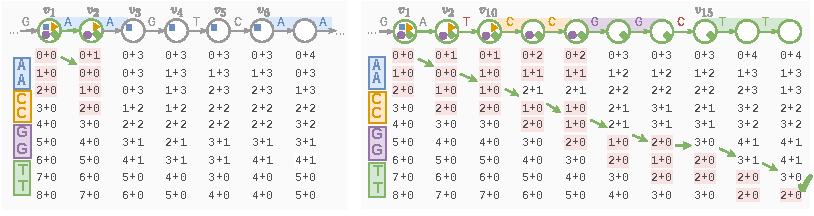
\includegraphics[width=\linewidth]{\dir/figures/seed-heuristic-tables}
	\caption{Exploration of $\AG[q]$, searching for a shortest path from the
	first to the last row using the \seedh. The table entry in the $i^\text{th}$
	row (zero indexed) below node $v$ shows $g\st{v}{i}+h\st{v}{i}$, where
	$g\st{v}{i}$ is the shortest distance from any starting state $\st{u}{0}$ to
	$\st{v}{i}$.
	%
	States that may\textsuperscript{\cref{SEEDfootnote:tie-braking}} be expanded by
	the \A~algorithm are highlighted in \colorbox{pink-highlight}{pink}, and the
	rest of the states are shown for completeness even though they are never
	expanded. The shortest path corresponding to the best alignment is shown
	with green arrows~(\textcolor{dark-green}{$\pmb{\rightarrow}$}).}
	%
	\label{SEEDfig:exploration-table}
\end{figure}


\paragraph{Guiding the search example}
%
\cref{SEEDfig:exploration-table} demonstrates how $h\st{v}{i}$ guides the
\A~algorithm towards the shortest path by showing which states may be
\colorbox{pink-highlight}{expanded} when using the \sh.
%
Specifically, the unique optimal alignment in \cref{SEEDfig:overview} starts from
node $v_{1}$, continues to $v_{2}$, and then proceeds through node $v_{10}$
(instead of~$v_{3}$).

While the \sh initially explores all states of the form $\st{v}{0}$ (we
discuss in \cref{SEEDsec:trie} how to avoid this by using a trie), it skips
expanding any state that involves nodes $v_{3}$--$v_{8}$. This improvement is
possible because all these explored states are penalized by the \sh by at
least $3$, while the shortest path of cost $2$ will be found before considering
states on nodes $v_{3}$--$v_{8}$.
%
Here, the heuristic function accurately predicts that expanding $v_{10}$ may
eventually lead to an exact alignment of seeds
\colorbox{light-yellow}{$\mathtt{CC}$}, \colorbox{light-violet}{$\mathtt{GG}$}
and \colorbox{light-green}{$\mathtt{TT}$}, while expanding $v_3$ may not lead to
an alignment of either seed.
%
In particular, the \sh is not misled by the short-term benefit of correctly
matching $A$ in $v_{2}$, and instead provides a long-term recommendation based
on the whole read. Thus, even though the walk to $v_{3}$ aligns exactly the
first two letters of $q$, \A does not expand $v_{3}$ because the \sh
guarantees that the future cost will be at least $3$.

% Overall, the \sh directs the search to the best alignment with one
% substitution
% ($\mathtt{\textcolor{dark-red}{T}{\rightarrow}\textcolor{dark-red}{A}}$) and
% one deletion ($\textcolor{dark-red}{\mathtt{C}}$).

\begin{figure}[H]
    \centering
%    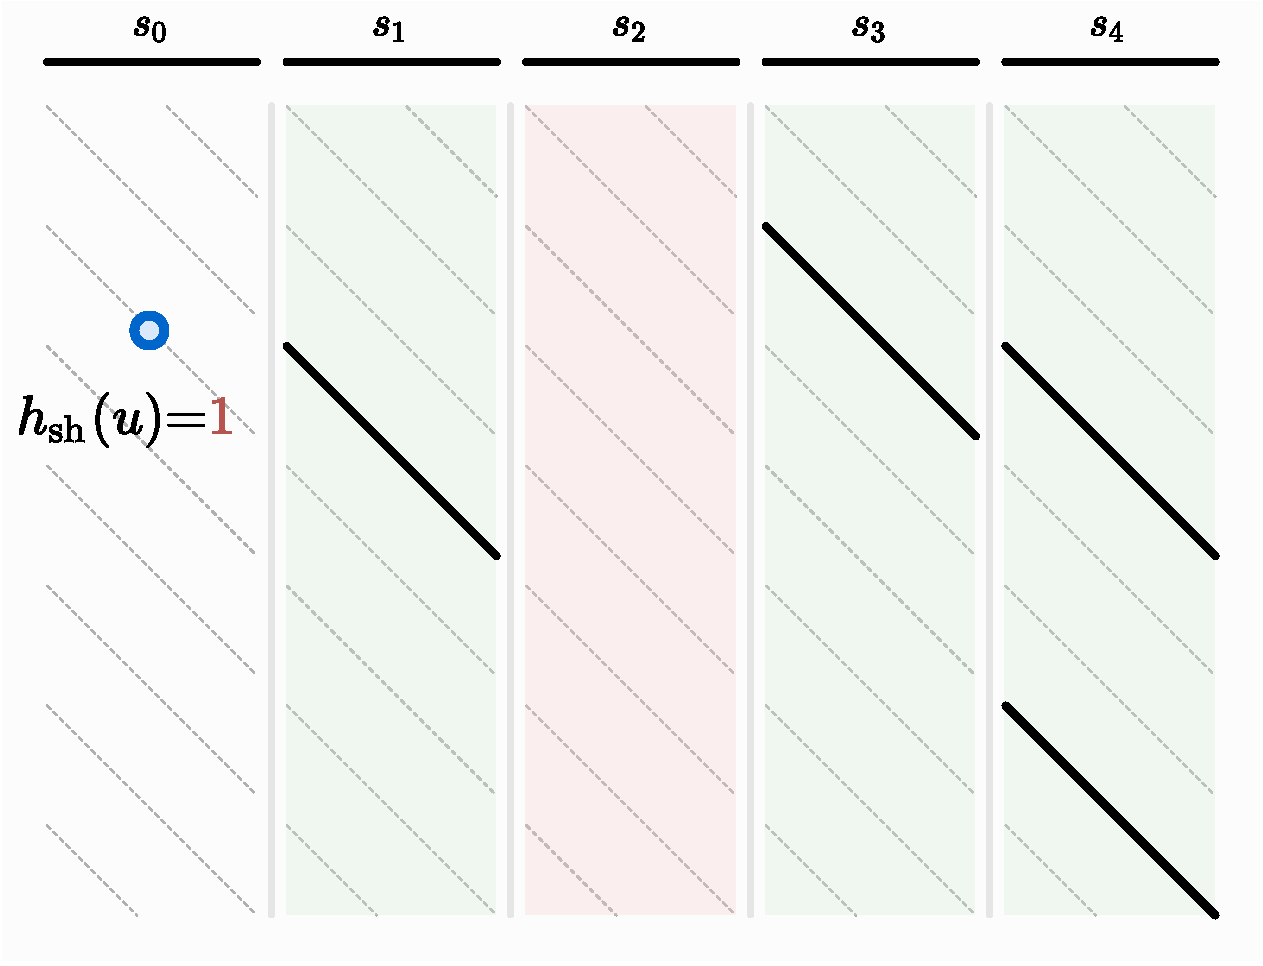
\includegraphics[width=0.24\linewidth]{imgs/heuristic-diagrams/sh.pdf}

    \subfloat[\Sh]{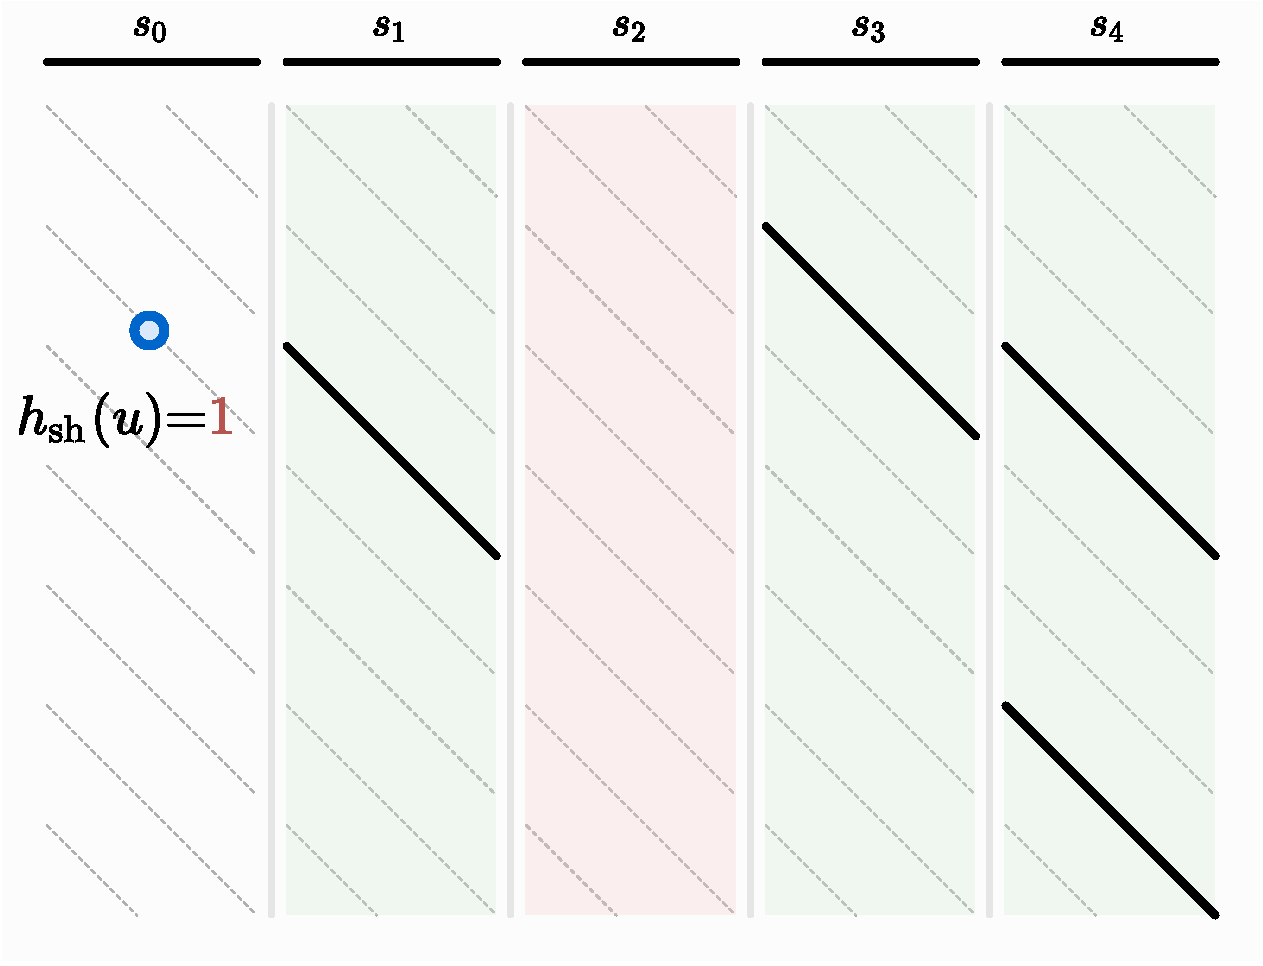
\includegraphics[width=0.4\linewidth]{imgs/heuristic-diagrams/sh.pdf}\label{fig:sh}}
    \hfill
    \subfloat[\Csh]{
\includegraphics[width=0.4\linewidth]{imgs/heuristic-diagrams/csh.pdf}\label{fig:csh}}
    \\ %\hfill
    \subfloat[\Gch]{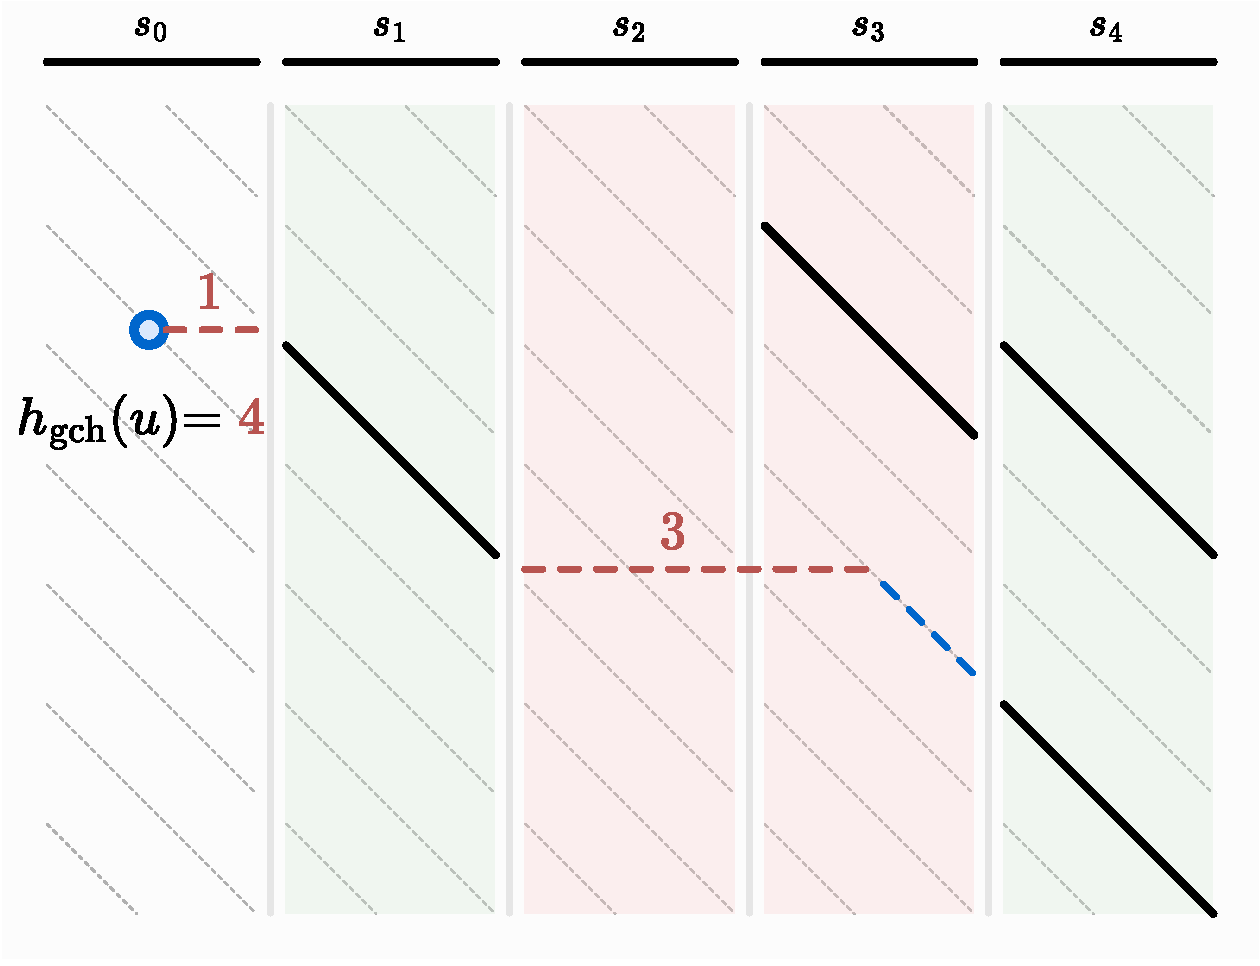
\includegraphics[width=0.4\linewidth]{imgs/heuristic-diagrams/gch.pdf}\label{fig:gch}}
    \hfill
    \subfloat[\CSH + match pruning]{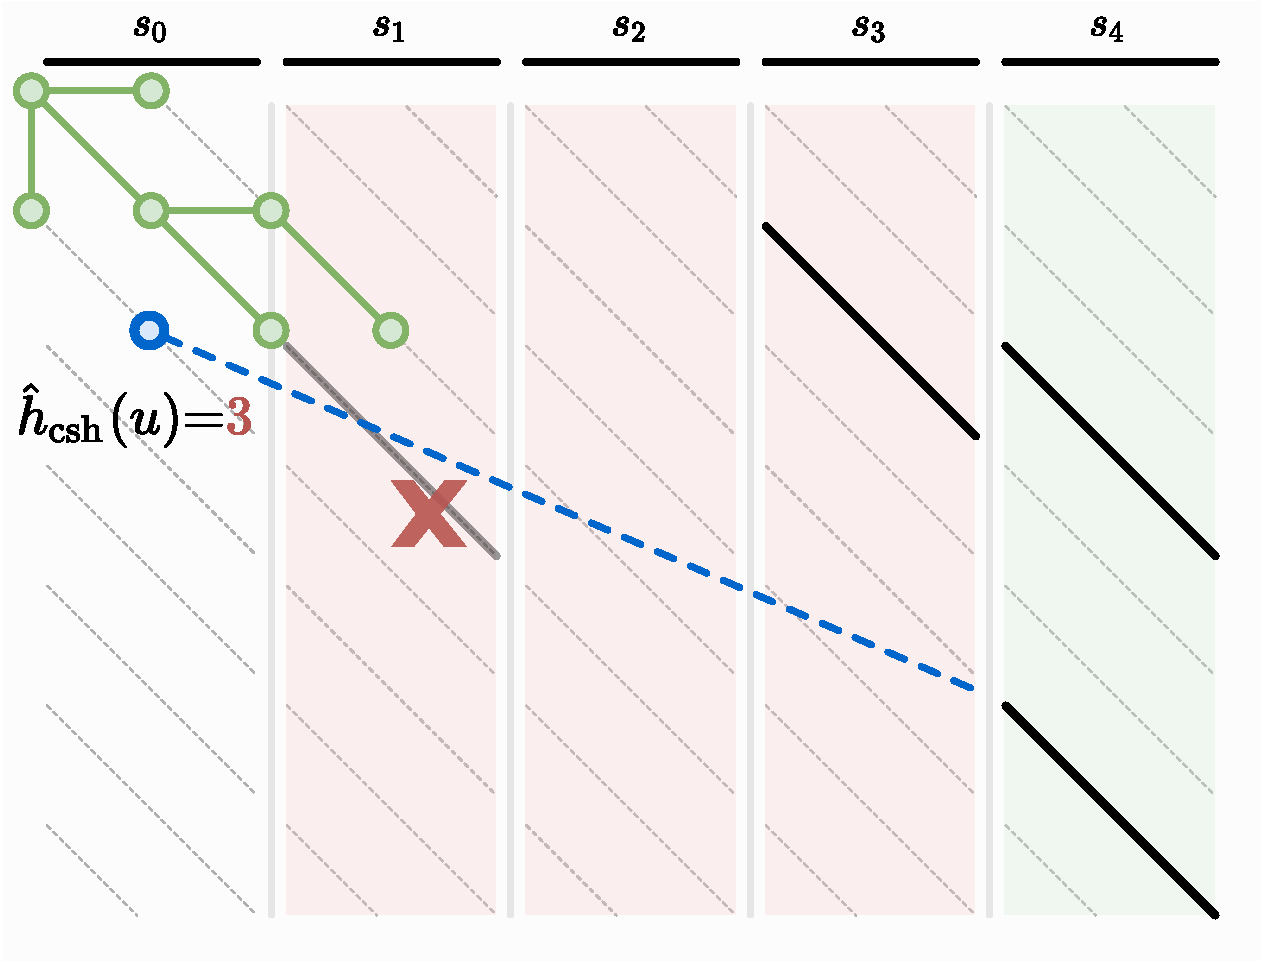
\includegraphics[width=0.4\linewidth]{imgs/heuristic-diagrams/pruning.pdf}\label{fig:pruning}}

    \caption[Family of chaining seed heuristics]{\textbf{Demonstration of \sh, \csh, \gch, and match pruning.}
      Sequence $A$ is split into $5$ seeds (horizontal black segments \seed) on
      top. Each seed is exactly matched in $B$ (diagonal black segments \match).
      The heuristic is evaluated at state $u$ (blue circles \bluecircle), based
      on the $4$ remaining seeds. The heuristic value is based on a maximal
      chain of matches (green columns \greencolumn\ for seeds with
      matches; red columns \redcolumn\ otherwise). Dashed lines denote chaining
      of matches.
      %
      \protect\subref{fig:sh} The \sh $\hsh(u) {=} 1$ is the number of remaining
      seeds that do not have matches (only $s_2$).
      %
      \protect\subref{fig:csh} The \csh $\hcsh(u) {=} 2$ is the number of
      remaining seeds without a match ($s_2$ and $s_3$) on a path going only
      down and to the right containing a maximal number of matches.
      %
      \protect\subref{fig:gch} The \gch $\hgch(u) {=} 4$ is minimal cost of a
      chain, where the cost of joining two matches is the maximum of the number
      of not matched seeds and the gap cost between them. Red dashed lines
      denote gap costs.
      %
      \protect\subref{fig:pruning} Once the start or end of a match is expanded
      (green circles \greencircle), the match is \emph{pruned} (red cross
      \cross), and future computations of the heuristic ignore it. $s_1$ is
      removed from the maximum chain of matches starting at $u$ so $\hcshS(u)$
      increases by~$1$.}
    \label{fig:heuristics}
\end{figure}

\section{Seed heuristic} \label{sec:seed_heuristic}
%
We instantiate the \A algorithm with a novel, domain-specific \textit{\seedh}
which allows to quickly align reads to a general reference graph.
%
We first intuitively explain the seed heuristic and showcase it on a simple
example (\cref{sec:overview}). Then, we formally define the heuristic and prove
its admissibility (\cref{sec:definition}).
%
Finally, we adapt our approach to rely on a trie, which leads to a critical
speedup (\cref{sec:trie}).

% This text will be sanitized and placed into lqa-output/abstract.txt
%
Motivation and approach: the trie index works for scaling sublinerly with the
reference size but each error in the query triggers deeper exploration of the
trie so the runtime grows exponentially. Lets inform the \A algorithm using
information from the whole query length while keeping the trie. This way we
could avoid the deep trie exploration and scale to long queries (as far as the
error rate is not too high).

We present a novel \A \emph{\seedh} that enables fast and optimal
sequence-to-graph alignment, guaranteed to minimize the edit distance of the
alignment assuming non-negative edit costs.

We phrase optimal alignment as a shortest path problem and solve it by
instantiating the \A~algorithm with our \seedh. The \seedh first extracts
non-overlapping substrings (\emph{seeds}) from the read, finds exact seed
\emph{matches} in the reference, marks preceding reference positions by
\emph{crumbs}, and uses the crumbs to direct the \A search. The key idea is to
punish paths for the absence of foreseeable seed matches. We prove admissibility
of the \seedh, thus guaranteeing alignment optimality.

\qquad Our implementation extends the free and open source aligner and
demonstrates that the \seedh outperforms all state-of-the-art optimal aligners
including \graphaligner, \vargas, \pasgal, and the \prefixh previously employed
by \astarix. Specifically, we achieve a consistent speedup of >60$\times$ on
both short Illumina reads and long HiFi reads (up to 25kbp), on both the
\textit{E.~coli} linear reference genome (1Mbp) and the MHC variant graph
(5Mbp). Our speedup is enabled by the \seedh consistently skipping >99.99\% of
the table cells that optimal aligners based on dynamic programming
compute.\\

\astarix aligner and evaluations: \astarixurl\\

Genome graph, Optimal alignment, Semi-global alignment, Edit distance, Shortest
path, Long reads, \A algorithm, Seed heuristic
\section{Overview}

% General: aligning, edit distance
Alignment of reads to a reference genome is an essential and early step in most
bioinformatics pipelines. While linear references have been used traditionally,
an increasing interest is directed towards graph references capable of
representing biological variation~\citep{garrison_variation_2018}.
%
Specifically, a \emph{sequence-to-graph} alignment is a base-to-base
correspondence between a given read and a walk in the graph. As sequencing
errors and biological variation result in inexact read alignments, edit distance
is the most common metric that alignment algorithms optimize in order to find
the most probable read origin in the reference.

% We note that in contrast to linear references, reference graphs capture
% genomic variation and therefore enable more accurate
% alignments~\citep{garrison_variation_2018}.

\paragraph{Suboptimal alignment}
%
In the last decades, approximate and alignment-free methods satisfied the demand
for faster algorithms which process huge volumes of genetic
data~\citep{kucherov2019evolution}. 
%
\emph{Seed-and-extend} is arguably the most popular paradigm in read
alignment~\citep{altschul_basic_1990,langmead_fast_2012,li_fast_2009}. First,
substrings (called \emph{seeds} or \emph{kmers}) of the read are extracted, then
aligned to the reference, and finally prospective matching locations are
\emph{extended} on both sides to align the full read.

While such a heuristic may produce acceptable alignments in many cases, it
fundamentally does not provide quality guarantees, resulting in suboptimal
alignment accuracy.
%
In contrast, here we demonstrate that seeds can benefit optimal alignment as
well.

\paragraph{Key challenges in optimal alignment}
%
Finding optimal alignments is desirable but expensive in the worst case,
requiring $\Oh(Nm)$ time~\citep{equi2019complexity}, for graph size $N$ and read
length $m$.
%
Unfortunately, most optimal sequence-to-graph aligners rely on dynamic
programming (DP) and always reach this worst-case asymptotic runtime. Such
aligners include \vargas~\citep{darby2020vargas},
\pasgal~\citep{jain_accelerating_2019},
\graphaligner~\citep{rautiainen_bitparallel_2019},
\hga~\citep{feng2021accelerating}, and \vg~\citep{garrison_variation_2018},
which use bit-level optimizations and parallelization to increase their
throughput.

In contrast, we follow the promising direction of using a heuristic to avoid
worst-case runtime on realistic data. To this end, \astarix rephrases the task
of alignment as a shortest-path problem in an \emph{alignment graph} extended by
a \emph{trie index}, and solves it using the \A~algorithm instantiated with a
problem-specific \prefixh. Importantly, its choice of heuristic only affects
performance, not optimality.
%
Unlike DP-based algorithms, this \prefixh allows scaling sublinearly with the
reference size, substantially increasing performance on large genomes. However,
it can only efficiently align reads of limited length.

\paragraph{Contributions}
%
Here we address the key challenge of scaling to long HiFi reads, while
retaining the superior scaling of \astarix in the size of the reference graph.
%
To this end, we instantiate the \A algorithm with a novel \seedh, which
outperforms existing optimal aligners on both short and long HiFi reads.
%
Specifically, the \seedh utilizes information from the whole read to narrowly
direct the \A search by placing \emph{crumbs} on graph nodes which lead up to a
\emph{seed match}, \ie, an exact match of a substring of the read.

Overall, the contributions presented next include:
\begin{enumerate}
    \item A novel \A~\seedh that exploits information from the whole read to
    quickly align it to a general graphs reference.
    \item An optimality proof showing that the \seedh always finds an alignment
    with minimal edit distance.
	\item An implementation of the \seedh as part of the \astarix aligner.
    \item An extensive evaluation of our approach, showing that we align both
    short Illumina reads and long HiFi reads to both linear and graph references
    $\geq 60 \times$ faster than existing optimal aligners.
    \item A demonstration of superior empirical runtime scaling in the reference
    size $N$: $N^{0.46}$ on Illumina reads and $N^{0.11}$ on HiFi reads.
\end{enumerate}

\input{\dir/figures/overview-figure.tex}

\paragraph{Intuition} \label{SEEDsec:overview}
% Task
\cref{SEEDfig:overview} showcases the \sh on an overview example. It shows a
read~$q$ to be aligned to a reference graph~$\RG$. Our goal is to find an
optimal alignment starting from an arbitrary node $v \in \RG$.
%
For simplicity of the exposition, we assume unit edit costs $\cedits =
(0,1,1,1)$, which we generalize in~\cref{SEEDsec:definition}.

\paragraph{Intuition}
The \A search requires us to provide a lower bound of the remaining path cost
from a state $\st{v}{i}$ to a target state. Clearly, to align the whole query,
each of the remaining seeds (\ie~at or after position $i$ in $q$) has to be
eventually aligned. The intuition underlying the \sh is to punish the state
for the absence of any foreseeable match of each remaining seed. Notice that the
order of the seeds is not directly taken into account.

In order to quickly check if a seed $s$ can lead to a match, we follow a
procedure similar to the one used by Hansel and Gretel who were placing
breadcrumbs to find their trail back home. Before aligning a query, we will
precompute all $\emph{crumbs}$ from all seeds so that not finding a crumb for
a seed $s$ on node $v$ indicates that seed $s$ could not be matched exactly
before the query is fully aligned continuing from $v$. This way, assuming that a
shortest path includes many seed matches, the crumbs will direct the \A search
along with it.

If a crumb from an expected seed is missing in node $v$, its corresponding seed
$s$ could not possibly be aligned exactly and this will incur the cost of at
least one substitution, insertion, or deletion. Assuming unit edit costs,
$h\st{v}{i}$ yields a lower bound on the cost for aligning $q[i{:}]$ starting
from $v$ by simply returning the number of missing expected crumbs in $v$.

\paragraph{Crumbs precomputation example}
%
\cref{SEEDfig:overview} shows four seeds as colored sections of length $2$ each, and
represents their corresponding crumbs as \bluecrumb{}, \yellowcrumb{},
\violetcrumb{} and \greencrumb{}, respectively. Four crumbs are expected if we
start at $v_2$, but \bluecrumb{} is missing, so $h\st{v_2}{0}=1$. Analogously,
if we reach $v_2$ after aligning one letter from the read, we expect 3 crumbs
(except \bluecrumb{}), and we find them all in $v_2$, so $h\st{v_2}{1}=0$.
%
To precompute the crumbs for each seed, we first find all positions in $\RG$
from which the seed aligns exactly. \cref{SEEDfig:overview} shows these exact
matches as colored sections of $\RG$. Then, from each match we traverse $\RG$
backwards and add crumbs to nodes that could lead to these matches.
%
For example, because seed \colorbox{light-yellow}{$\mathtt{CC}$} can be matched
starting in node $v_{10}$, crumbs~\yellowcrumb{} are placed on all nodes leading
up to $v_{10}$.
%
Similarly, seed \colorbox{light-blue}{$\mathtt{AA}$} has two exact matches, one
starting in node $v_{0}$ and one starting in node $v_{6}$.
%
However, we only add crumbs \bluecrumb{} to nodes $v_{0}$, $v_{1}$, and
$v_{3}$--$v_{6}$, but not to node $v_{2}$. This is because $v_{2}$ is
(i)~strictly after the beginning of the match of
\colorbox{light-blue}{$\mathtt{AA}$} at $v_1$ and (ii)~too far before the match
of \colorbox{light-blue}{$\mathtt{AA}$} at $v_{6}$.
%
Specifically, any alignment starting from node $v_{2}$ and still matching
\colorbox{light-blue}{$\mathtt{AA}$} at $v_{6}$ would induce an overall cost of
$4$ (it would require deleting the $4$ letters $A$, $G$, $T$, and $C$). Even
without a crumb \bluecrumb{} on $v_{2}$, our heuristic provides a lower bound on
the cost of such an alignment: it never estimates a cost of more than~$4$, the
number of seeds.

% In contrast to \bluecrumb{}, the crumbs \greencrumb{} for the match of seed
% \colorbox{light-green}{$\mathtt{TT}$} are placed on all nodes before $v_{15}$.
% This is because even when starting from $v_0$, we could match
% \colorbox{light-green}{$\mathtt{TT}$} at $v_{15}$ without a cost exceeding the
% cost of $4$ (by deleting $\mathtt{G}$, substituting
% $\mathtt{\textcolor{dark-red}{T}{\rightarrow}\textcolor{dark-red}{A}}$, and
% deleting $\mathtt{\textcolor{dark-red}{C}}$, at an overall cost of $3$).

\input{\dir/figures/exploration-table-figure.tex}

\paragraph{Guiding the search example}
%
\cref{SEEDfig:exploration-table} demonstrates how $h\st{v}{i}$ guides the
\A~algorithm towards the shortest path by showing which states may be
\colorbox{pink-highlight}{expanded} when using the \sh.
%
Specifically, the unique optimal alignment in \cref{SEEDfig:overview} starts from
node $v_{1}$, continues to $v_{2}$, and then proceeds through node $v_{10}$
(instead of~$v_{3}$).

While the \sh initially explores all states of the form $\st{v}{0}$ (we
discuss in \cref{SEEDsec:trie} how to avoid this by using a trie), it skips
expanding any state that involves nodes $v_{3}$--$v_{8}$. This improvement is
possible because all these explored states are penalized by the \sh by at
least $3$, while the shortest path of cost $2$ will be found before considering
states on nodes $v_{3}$--$v_{8}$.
%
Here, the heuristic function accurately predicts that expanding $v_{10}$ may
eventually lead to an exact alignment of seeds
\colorbox{light-yellow}{$\mathtt{CC}$}, \colorbox{light-violet}{$\mathtt{GG}$}
and \colorbox{light-green}{$\mathtt{TT}$}, while expanding $v_3$ may not lead to
an alignment of either seed.
%
In particular, the \sh is not misled by the short-term benefit of correctly
matching $A$ in $v_{2}$, and instead provides a long-term recommendation based
on the whole read. Thus, even though the walk to $v_{3}$ aligns exactly the
first two letters of $q$, \A does not expand $v_{3}$ because the \sh
guarantees that the future cost will be at least $3$.

% Overall, the \sh directs the search to the best alignment with one
% substitution
% ($\mathtt{\textcolor{dark-red}{T}{\rightarrow}\textcolor{dark-red}{A}}$) and
% one deletion ($\textcolor{dark-red}{\mathtt{C}}$).

\subsection{Formal definition of the seed heuristic with crumbs} \label{SEEDsec:definition}
%
Next, we formally define the \seedh function $h\st{v}{i}$. Overall, we want to
ensure that $h\st{v}{i}$ is admissible, \ie, that it is a lower bound on the
cost of a shortest path from $\st{v}{i}$ to some $\st{w}{|q|}$ in $\AG$.

\paragraph{Seeds}
%
We split read $q \in \Sigma^*$ into a set $\seeds$ of non-overlapping seeds
$s_0, \dots, s_{|\seeds|-1} \in \Sigma^*$.
%
For simplicity, we assume that all seeds have the same length and are
consecutive, \ie, we split $q$ into substrings $s_0 \cdot s_1 \cdots
s_{|\seeds|-1} \cdot t$, where all $s_j$ are seeds of length $k$ and we ignore
the suffix $t$ of $q$, which is shorter than~$k$.
%
We note that our approach could be trivially generalized to seeds of different
lengths or non-consecutive seeds as long as they do not overlap. An interesting
future work item is investigating how different choices of seeds affect the
performance of our approach, and selecting seeds accordingly.

\paragraph{Matches}
%
For each seed $s \in \seeds$, we locate all nodes $u \in M(s)$ in the reference
graph that can be the start of an exact match of $s$:
%
\begin{align*}
	M(s) := \{u \in \RGV \mid \exists \text{walk } \pi \text{ starting from } u \in \RG \text{ and spelling } \sigma(\pi) = s \}.
\end{align*}
%
To compute $M(s)$ efficiently, we leverage the trie introduced in
\cref{SEEDsec:trie}.

\paragraph{Crumbs}
For seed $s_j$ starting at position $i$ in $q$, we place crumbs on all nodes $u
\in \RGV$ which can reach a node $v \in M(s_j)$ using less than $i+\maxdel$
edges:
%
\begin{align*}
	C(s) := \{u \in \RGV \mid & \exists v \in M(s)\colon \mli{dist}(u, v) < i + \maxdel \},\\
	\text{where }\mli{dist}(u, v) &\text{ is the length of a shortest walk from } u \text{ to } v.
\end{align*}

Later in this section, we will select $\maxdel$ to ensure that if an alignment
uses more than $\maxdel$ deletions, its cost must be so high that the heuristic
function is trivially admissible.

To compute $C(s)$ efficiently, we can traverse the reference graph backwards
from each $v \in M(s)$ by a backward breadth-first-search (BFS).

% Crumbs should be placed before each exact match so that any alignment that may
% reach the match sees a crumb. For each seed we calculate the maximal distance
% to a match that has to be covered by crumbs. More specifically, we compute
% this distance as $i{+}d$, where $i$ is the position of the seed in the read
% (seeds towards the end need more crumbs so that the beginning of the alignment
% can also see them), and $d$ is the maximal number of deletions (since a
% deletion in the read may require a longer alignment in the reference grap)
% after which the \seedh is anyway capped.\todo{explain better} Note that
% putting crumbs in all nodes that can potentially lead to an exact match is
% crucial for the optimality guarantees of the \seedh, while putting unnecessary
% crumbs may only make the heuristic less precise so more state may be explored.
% So in~\cref{SEEDthe:admissible} we prove that all necessary crumbs are placed and
% the heuristic is admissible.

\paragraph{Heuristic}
%
Let $\seeds_{\ge i}$ be the set of seeds that start at or after position $i$ of
the read, formally defined by $\seeds_{\ge i} := \{s_{j} \mid \lceil i / k
\rceil \leq j < |\seeds|  \}$.
%
This allows us to define the number of expected but missing crumbs in state
$\st{v}{i}$ as $\mli{misses}\st{v}{i} := \big\lvert \left\{  s
\in \seeds_{\ge i} \mid v \notin C(s) \right \} \big\rvert$.
%
Finally, we define the \seedh as
\begin{align} \label{SEEDeq:heuristic}
	h\st{v}{i} &= (\lvert q \rvert - i) \cdot \cmatch + \mli{misses}\st{v}{i} \cdot \delta_\mli{min},\\
	\text{for } &\delta_\mli{min} = \min(\csubst - \cmatch,\cdel,\cins - \cmatch), \label{SEEDeq:delta}
\end{align}
%
Intuitively, \cref{SEEDeq:heuristic} reflects that the cost of aligning each
remaining letter from $q[i{:}]$ is at least $\cmatch$. In addition, every
inexact alignment of a seed induces an additional cost of at least
$\delta_\mli{min}$. 
%
Specifically, every substitution costs $\csubst$ but requires one less match;
every deletion costs $\cdel$; and every insertion costs $\cins$ but also
requires one less match.

We note that $h\st{v}{i}$ implicitly also depends on the reference graph $\RG$,
the read $q$, the set of seeds, and the edit costs $\cedits$.

In order for an alignment with at least $\maxdel$ deletions to have a cost so
high that the heuristic function is trivially admissible, we ensure $\maxdel
\cdot \cdel \geq h\st{v}{i}$ by defining
\begin{align} \label{SEEDeq:maximum-deletions}
	\maxdel := \left\lceil \frac{\lvert q \rvert \cdot \cmatch + |\seeds| \cdot \delta_{\mli{min}}}{\cdel} \right\rceil.
\end{align}
%
In \cref{SEEDthe:admissible}, we show that $h\st{v}{i}$ is admissible, ensuring that
our heuristic yields optimal alignments.


\begin{thm}[Admissibility]
	\label{SEEDthe:admissible}
	The \seedh $h\st{v}{i}$ is admissible.
\end{thm}
\begin{proof}
	Let $A$ be an optimal alignment of $q[i{:}]$ starting from $v \in \RG$. We
	will prove that the cost of $A$ is at least $h\st{v}{i}$.

	If $A$ contains at least $\maxdel$ deletions, its cost is at least $\maxdel
	\cdot \cdel$, which is at least $|q| \cdot \cmatch + |\seeds| \cdot
	\delta_{\mli{min}}$ by plugging in $\maxdel$ from
	\cref{SEEDeq:maximum-deletions}. This is an upper bound for $h\st{v}{i}$, which
	we observe after maximizing $h\st{v}{i}$ by substituting $i=1$ and
	$\mli{misses}=|\seeds|$ into~\cref{SEEDeq:heuristic}, which concludes the proof
	in this case.

	Otherwise, $A$ contains less than $\maxdel$ deletions.
	%
	If we interpret $A$ as a path in $\AG$, we first observe that $A$ must spell
	$q[i{:}]$. Thus, $A$ must in particular also contain all seeds $s_j \in
	\seeds_{\geq i}$ as substrings. We then split $A$ into \emph{subalignments}
	$A_{-1}, A_0, \dots, A_{p}$, selected such that $A_0, \dots, A_{p-1}$ spell
	the seeds $s_j \in \seeds_{\geq i}$, and $A_{-1}$ and $A_p$ spell the prefix
	and suffix of $q[i{:}]$ which do not cover any full seed.

	This ensures that we can compute a lower bound on the cost of $A$ as
	follows:
	\begin{align}
		\text{cost}(A) 
		&= \sum_{j=-1}^{p} \text{cost}(A_k) \label{SEEDeq:split-cost} \\
		&\geq \sum_{j=-1}^{p} \lvert \sigma(A_k) \rvert \cdot \cmatch + \sum_{j=0}^{p-1} \left\{ \begin{array}{ll}
			0 & \text{ if } v \in C\!\left(s_{\left\lceil i/k \right\rceil + j}\right) \\
			\delta_\mli{min} & \text{ if } v \notin C\!\left(s_{\left\lceil i/k \right\rceil + j}\right)
		\end{array}\right\} \label{SEEDeq:rearrange-cost} \\
		&= (\lvert q \rvert - i) \cdot \cmatch + \big\lvert \{v \notin C(s) \mid s \in \seeds_{\geq i}\} \big\rvert \cdot \delta_\mli{min} \label{SEEDeq:various} \\
		&= h\st{v}{i} \label{SEEDeq:plug-in-heuristic}
	\end{align}
	%
	Here, \cref{SEEDeq:split-cost} follows from our decomposition of $A$. If we
	ignore the right-hand side in \cref{SEEDeq:rearrange-cost} (right of ``$+$''),
	the inequality follows because matching all letters is the cheapest method
	to align any string. The right-hand side follows from a more precise
	analysis for subalignments $A_k$ that spell a seed $s_{\left\lceil i/k
	\right\rceil + j}$ without a corresponding crumb in $v$. The absence of such
	a crumb indicates that no exact match of $s_{\left\lceil i/k \right\rceil +
	j}$ in $\RG$ can be reached within less than $i + \maxdel$ steps from $v$.
	However, because $A$ contains less than $\maxdel$ deletions, $A_k$ must
	start within less than $i + \maxdel$ steps from $v$. Thus, $A_k$ does not
	align $s_{\left\lceil i/k \right\rceil + j}$ exactly, meaning that it
	introduces a cost of at least $\delta_\mli{min}$.

	\cref{SEEDeq:various} follows from observing that $A_{-1}, \dots, A_p$ have a
	total length of $|q|-i$, and observing that the right-hand sum adds up
	$\delta_{\mli{min}}$ for every expected but missing crumb.
	%
	Finally, \cref{SEEDeq:plug-in-heuristic} follows from our definition of
	$h\st{v}{i}$, concluding the proof.
	%
\end{proof}

%\begin{algorithm}[H]
	\caption{For each seed: find all its exact matches in the reference graph
	and put corresponding crumbs backwards from the match. \todo{make the code not exponential like SeedStarts} \todo{SeedStarts in $O(n^2)$}}\label{alg:crumbs}
	\begin{algorithmic}[1]
		\State \makebox[0.4in][r]{$\RG\colon$} Reference graph \label{lin:reference}
        \State \makebox[0.4in][r]{$l\colon$} Length of each seed
		\State \makebox[0.4in][r]{$C(s)\colon$} Set of nodes with a crumb for seed $s$
        \State \makebox[0.4in][r]{$\maxdel\colon$} Maximum number of deletions\label{lin:d}
		\Comment{defined in \cref{eq:maximum-deletions}}
		\Statex
		\Function{PlaceAllCrumbs}{$q\colon$ Read}
			\State $S \gets \{\, q[kl {:} kl+l] \mid k \in \mathbb{N}, kl+l \leq \lvert q \rvert \}$
            \Comment{Split $q$ into seeds} \label{lin:seeds}
			\ForAll{$s \in S$} \label{lin:seeds-loop}
				\State $C(s) \gets \emptyset$ \label{lin:clear-crumbs}
				\ForAll{$u \in \Call{SeedStarts}{s}$} \label{lin:seed-starts-call}
					\State $i \gets \mli{start}(s)$
					\Comment{Starting position of $s$ in $q$} \label{lin:start}
					\State $\Call{PlaceCrumbsBackwards}{s, u, i + \maxdel}$
					\Comment{Crumbs on nodes before $u$} \label{lin:place-crumbs-backwards-call}
				\EndFor
			\EndFor
		\EndFunction
		\Statex
		\Function{SeedStarts}{$s\colon$ Seed}
			\State $T \gets \RGV$
			\Comment{Start from all nodes}
			\label{lin:match-init}
        	\ForAll{$k \in [0, \dots, l-1 ]$}
			\Comment{Match seed letters forward}
			\label{lin:match-forward-start}
				\State $T \gets \{w \mid v \in T, (v, w, s[k]) \in \RGE\}$
				\Comment{Follow edges matching $s[k]$ (forward)}
			\EndFor \label{lin:match-forward-end}
        		\ForAll{$k \in [l-1, \dots, 0 ]$}
				\Comment{Match seed letters backward}
				\label{lin:match-backward-start}
					\State $T \gets \{u \mid v \in T, (u,v,s[k]) \in \RGE \}$
					\Comment{Follow edges matching $s[k]$ (backward)}
			\EndFor \label{lin:match-backward-end}
			\State $M(s) \gets T$
			\State \Return{$M(s)$}
		\EndFunction
		\Statex
		\Function{PlaceCrumbsBackwards}{$s \colon$Seed, $u \colon $Node, $k \colon $Number of
		edges} \label{lin:place-crumbs-backwards-start}
			\ForAll{$t \in \Call{BackwardsBFS}{u, k}$}
				\Comment Nodes $t$ reaching $u$ within $k$ edges
				\label{lin:backwards-bfs}
				\State $C(s) \gets C(s) \cup \{t\}$
				\Comment Add a crumb for seed $s$ to node $t$ \label{lin:place-crumbs-backwards-end}
			\EndFor
		\EndFunction
	\end{algorithmic}
\end{algorithm}

\subsection{Computing the Seed heuristic} \label{SEEDsec:algo}
%
In order to efficiently evaluate the \seedh $h\st{v}{i}$, we must be
able to compute the crumbs that should be associated with each vertex $v \in
\RGV$.
%
To this end, \textsc{PlaceAllCrumbs} in \cref{SEEDalg:crumbs} shows an efficient
algorithm for precomputing the crumbs $C(s_j)$.

\para{Place Crumbs}
\crefrange{lin:seeds}{lin:seeds-loop} loop over all seeds $s$.
\cref{SEEDlin:clear-crumbs} erases the crumbs placed for seed $s$ during the
alignment of previous reads, thus ensuring that the crumbs of previous
alignments do not affect the current run. Then, \cref{SEEDlin:seed-starts-call}
locates all exact matches of $s$ in $\RG$ by calling \textsc{SeedStarts}.
\textsc{SeedStarts} proceeds in two phases.
\crefrange{lin:match-init}{lin:match-forward-end} locate all nodes that can be
the end point of an exact match. Then,
\crefrange{lin:match-backward-start}{lin:match-backward-end} backtrack through
the graph, locating all nodes that can be the starting point of an exact match.
We note that \crefrange{lin:match-forward-start}{lin:match-forward-end} could be
omitted without jeopardizing the correctness of \textsc{SeedStarts}, but they
will be crucial when we introduce our trie optimization in \cref{SEEDsec:trie}.

For each node $u$ that can be the start of an exact match of $s$,
\cref{SEEDlin:place-crumbs-backwards-call} calls \textsc{PlaceCrumbsBackwards},
which places crumbs on all nodes before $u$, up to a distance of $i{+}d$. Here,
$i$ is the index of $s$ in $q$ (\cref{SEEDlin:start}), and $\maxdel$ is the maximum
number of deletions we tolerate (\cref{SEEDlin:d}).
%
In order to avoid repeatedly placing crumbs on the same nodes,
\textsc{PlaceCrumbsBackwards} internally uses a breath first search (BFS, see
\cref{SEEDlin:backwards-bfs}) starting from $u$ and proceeding through reverse edges
until depth $i + \maxdel$.
\begin{figure}[t]
    \centering
	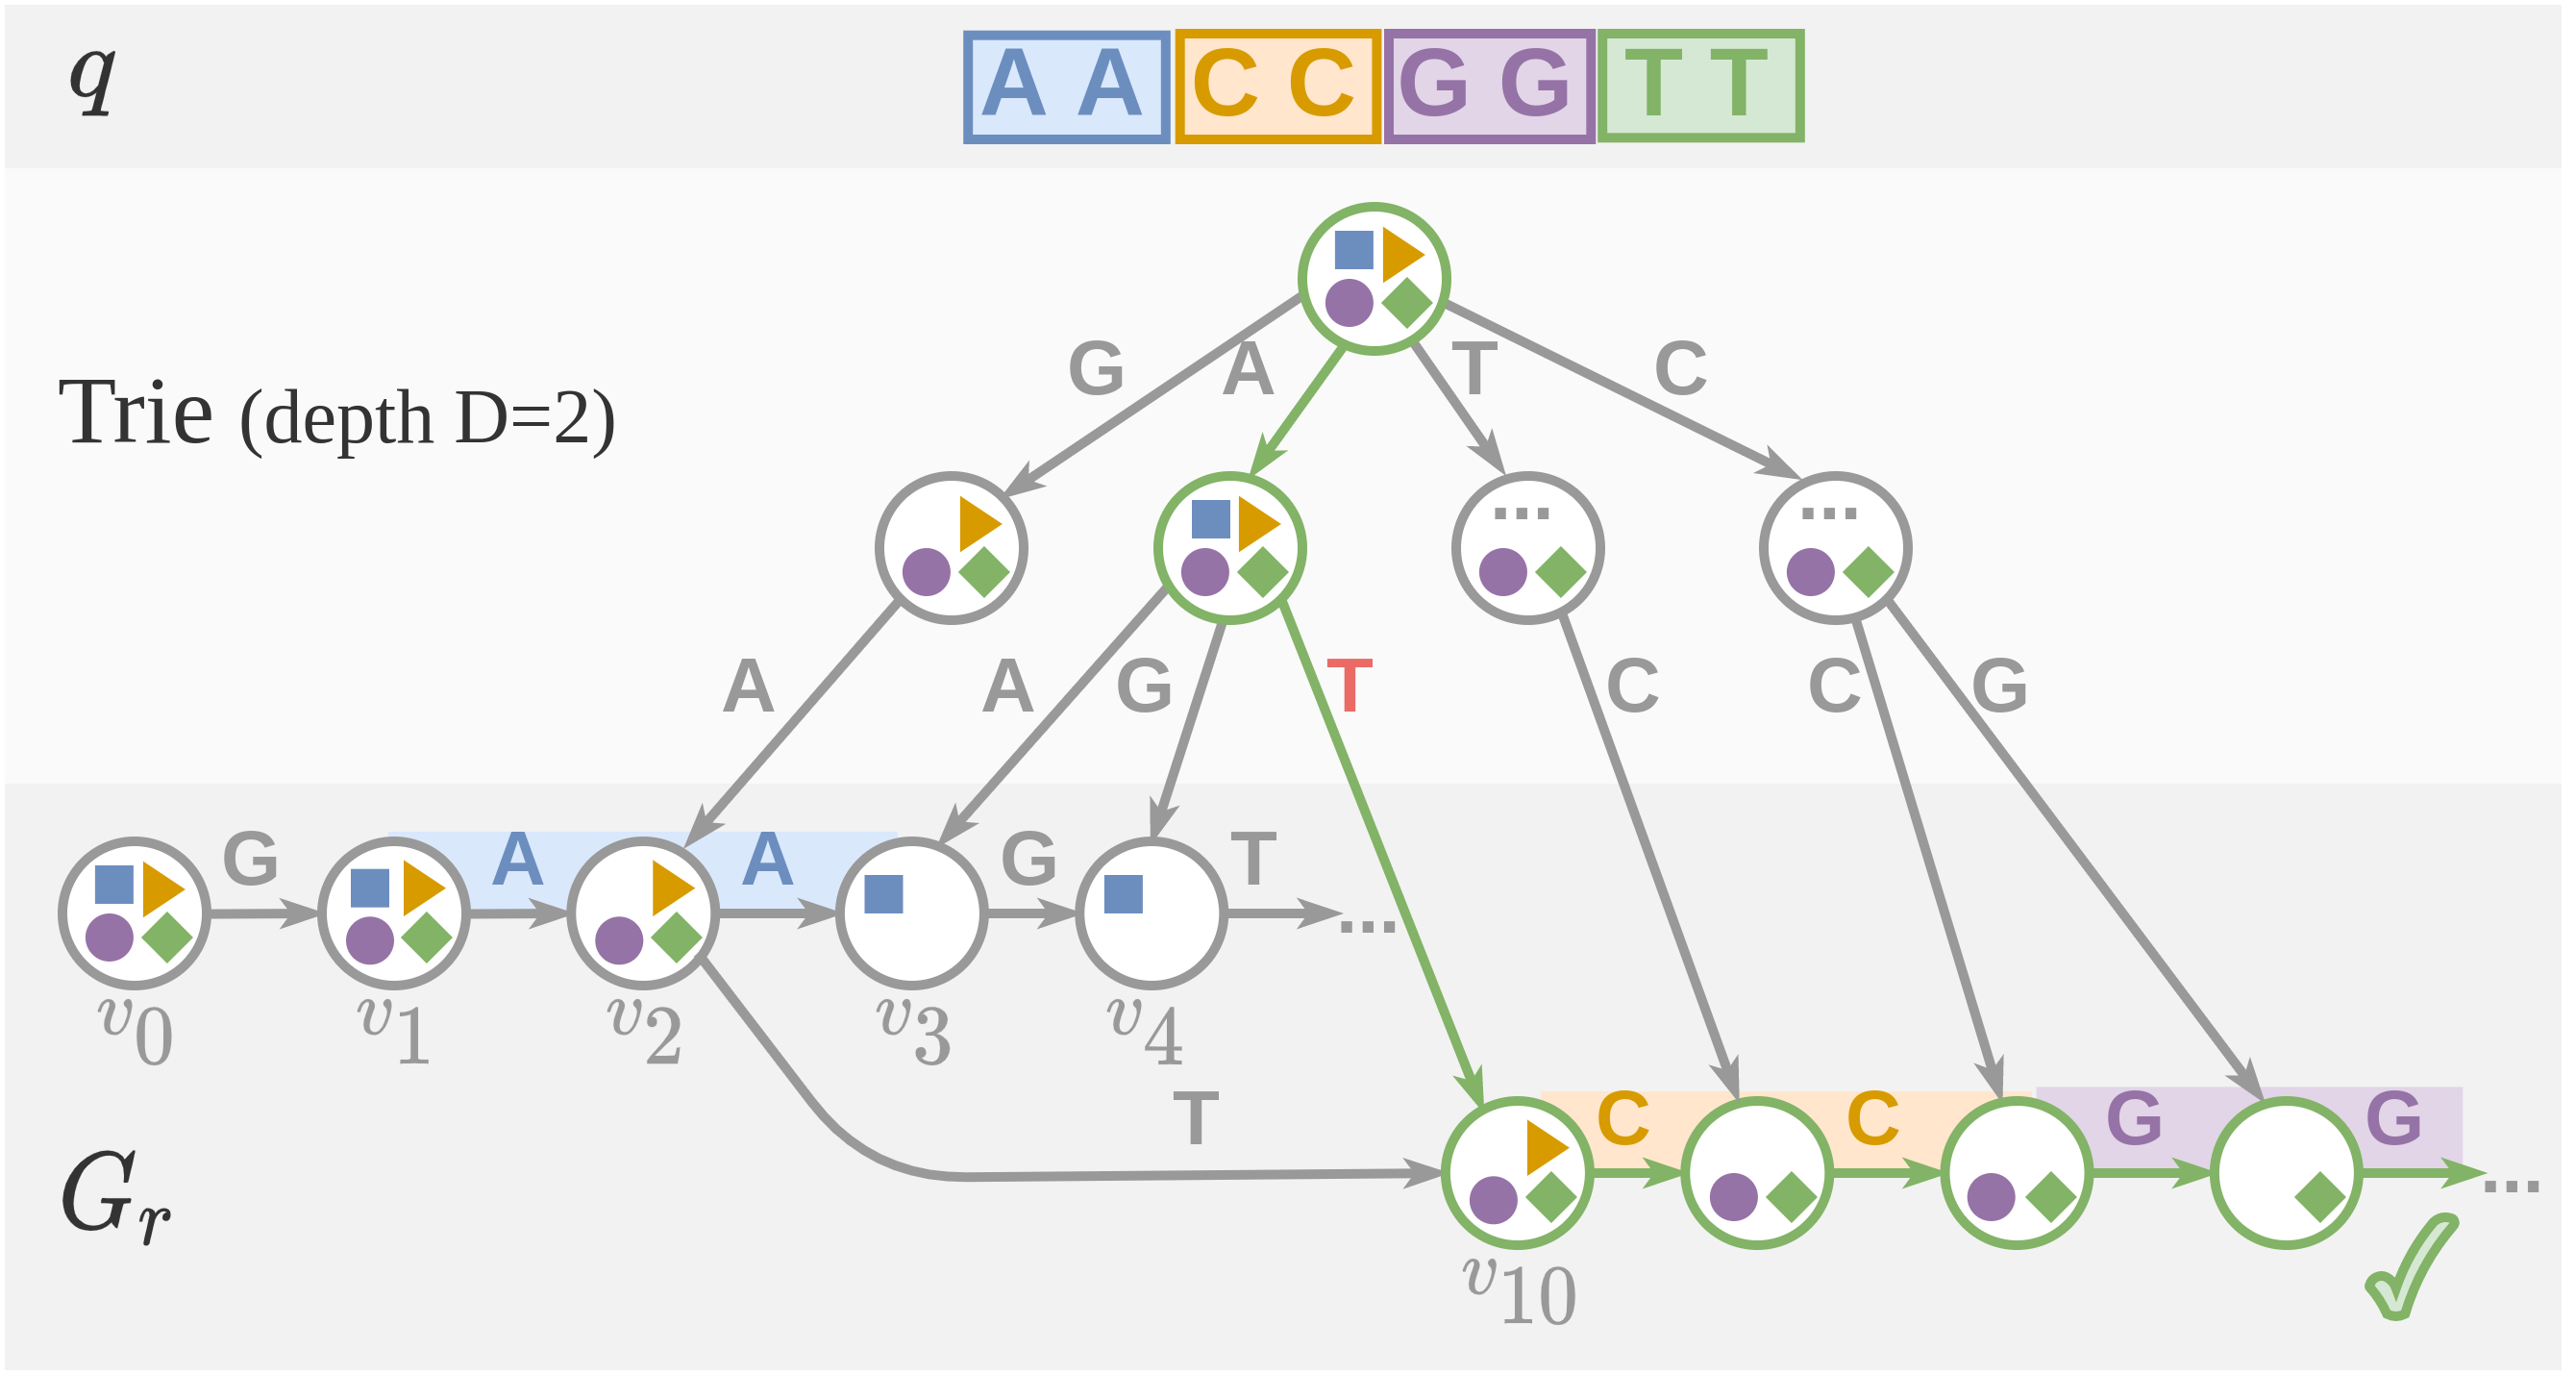
\includegraphics[width=0.6\linewidth]{figures/crumbs-trie.png}
	\caption{Reference graph from \cref{fig:overview}, extended by a trie of
	depth $D=2$. For simplicity, the reverse-complement reference graph and
	parts marked by ``\dots'' are omitted.}
	\label{fig:trie}
\end{figure}

\subsection{Trie index} \label{SEEDsec:trie}
%
Considering all nodes $v \in \RGV$ as possible starting points for the alignment
means that the \A~algorithm would explore all states of the form $\st{v}{0}$,
which immediately induces a high overhead of $\lvert \RGV \rvert$.
%
In line with previous works~\citep{ivanov2020astarix,dox2018efficient}, we avoid
this overhead by complementing the reference graph with a trie index to produce
a new graph $\TG = (\TGV, \TGE)$, where $\TGV$ is the union of the reference
graph nodes $\RGV$ and the new trie vertices, and $\TGE$ is the union of $\RGE$,
the trie edges, and edges connecting the trie leafs with reference nodes. Note
that constructing this trie index is a one-time pre-processing step that can be
reused for multiple queries.

Since we want to also support aligning reverse-complement reads by starting from
the trie \trieroot{}, we build the trie not only from the original reference
graph and also from its reverse-complement.

\para{Intuition}
%
\cref{SEEDfig:trie} extends the reference graph $\RG$ from \cref{SEEDfig:overview} with
a trie. Here, any path in the reference graph uniquely corresponds to a path
starting from the trie \trieroot{} (the top-most node in \cref{SEEDfig:trie}). Thus,
in order to find an optimal alignment, it suffices to consider paths starting
from the trie \trieroot{}, by using state $\st{\trieroot}{0}$ as the only source
for the \A~algorithm.
%
Note that if the reference graph branches frequently, the number of paths with
length $D$ may rise exponentially, leading to an exponential number of trie
leaves. To counteract this exponential growth, we can select $D$ logarithmically
small, as $\log_4N$.

For a more thorough introduction to the trie and its construction,
see~\citep{ivanov2020astarix}. Importantly, our placement of
crumbs~(\cref{SEEDsec:definition}) generalizes directly to reference graphs extended
with a trie (see also \cref{SEEDfig:trie}).

% This leads to the effect that the crumbs in a trie node correspond to the
% union of the crumbs of its descendents (with the exception when crumbs are
% skipped for propagating to the trie \cref{SEEDpara}).

\para{Reusing the trie to find seed matches}
%
As a second usage of the trie, we can also exploit it to efficiently locate all
matches $M(s)$ of a given seed $s$.
%
In order to find all nodes where a seed match begins, we align (without errors)
$\bar{s}$, the reverse-complement of $s$. To this end, we follow all paths
spelling $\bar{s}$ starting from the $\trieroot$---the final nodes of these
paths then correspond to nodes in $M(s)$. We ensure that the seed length $|s|$
is not shorter than the trie depth $D$, so that matching all letters in
$\bar{s}$ ensures that we eventually transition from a trie leaf to the
reference graph.

% Analogously, our computation of crumbs (\cref{SEEDsec:algo} and \cref{SEEDalg:crumbs})
% generalizes directly to reference graphs extended by a trie.
% %
% However, assuming that we select the depth of the trie to be the same as the
% length of each seed ($D=k$) allows us to speed up the computation by only
% starting the search for matches of a seed in~$\varepsilon$.
% %
% Specifically, in \cref{SEEDalg:crumbs}, we can replace \cref{SEEDlin:match-init} by $T
% \gets \{\varepsilon\}$. This is because
% \crefrange{lin:match-forward-start}{lin:match-forward-end} will locate all nodes
% in the original reference graph which can be the end point of a seed match.
% Then, \crefrange{lin:match-backward-start}{lin:match-backward-end} will
% backtrack both in the reference graph as well as in the trie, thus ensuring that
% $M(s)$ is computed correctly.

\para{Optimization: skip crumbs on the trie} \label{SEEDpar:skip_crumbs}
%
Generally, we aim to place as few crumbs as possible, in order to both reduce
precomputation time and avoid misleading the \A~algorithm by unnecessary crumbs.
In the following, we introduce an optimization to avoid placing crumbs on trie
nodes that are ``too close'' to the match of their corresponding seed so they
cannot lead to an optimal alignment.

Specifically, when traversing the reference graph backwards to place crumbs for
a match of seed $s$ starting at node $w$, we may ``climb'' from a reference
graph node $u$ to a trie node $u'$ backwards through an edge that otherwise
leads from the trie to the reference.
%
Assuming $s$ starts at position $i$ in the read, we have already established
that we can only consider nodes $u$ that can reach $w$ with less than
$i+\maxdel$ edges (see \cref{SEEDsec:definition}).
%
Here, we observe that it is sufficient to only climb into the trie from nodes
$u$ that can reach $w$ using more than~$i-\maxins-D$ edges, for
\begin{align}
	\maxins := \left\lceil \frac{\lvert q \rvert \cdot \cmatch + |\seeds| \cdot \delta_{\mli{min}}}{\cins} \right\rceil.
\end{align}
%
We define $\maxins$ analogously to $\maxdel$ to ensure that $\maxins$ insertions
will induce a cost that is always higher than $h\st{u}{i}$. We note that we can
only avoid climbing into the trie if all paths from $u$ to $w$ are too short, in
particular the longest one.

The following \cref{SEEDlem:trie-optimization} shows that this optimization
preserves optimality.

\begin{lem}[Admissibility when skipping crumbs]
	\label{SEEDlem:trie-optimization}
	The \seedh remains admissible when crumbs are skipped in the trie.
\end{lem}
\begin{proof}
	Consider a reference graph with a match of seed $s$ starting in node $w$.
	Now, consider a node $v$ that cannot reach $w$ using more than $i-D-\maxins$
	edges.
	%
	We can then show that a trie node $v'$ with a path to $v$ does not require a
	crumb for the match of $s$ in node $w$.

	Specifically, any path from $\trieroot$ through nodes $v'$ and $v$ to node
	$w$ has total length greater or equal $i-\maxins$. Thus, matching $s$ at $w$
	requires at least $\maxins$ insertions. Hence, the cost of such a path is at
	least $\maxins \cdot \cins = |q| \cdot \cmatch + n \cdot
	\delta_{\mli{min}}$. Observing that this is an upper bound for $h\st{v}{i}$
	concludes the proof.
	%
	\qedwhite
\end{proof}

In order to efficiently identify all nodes $u$ that can reach $w$ by using more
than $i-D-\maxins$ edges (among all nodes at a backward-distance at most
$i+\maxdel$ from $w$), we use topological sorting: considering only nodes at a
backward-distance at most $i+\maxdel$ from $w$, the length of a longest path
from a node $v$ to $w$ is (i)~$\infty$ if $v$ lies on a cycle and
(ii)~computable from nodes closer to $w$ otherwise.

\section{Algorithm} \label{GLOBALsec:computation}

\renewcommand\theenumi{\algletter\arabic{enumi}}
\renewcommand\labelenumi{{\rmfamily \algletter\arabic{enumi}.}}
\setlength{\leftmargini}{2em}

The algorithm we present here computes the shortest path in the alignment graph
using a variant of \A that handles pruning (\cref{GLOBALsec:astar}). This
depends on the efficient computation of the heuristics
(\cref{GLOBALsec:compute-sh,GLOBALsec:compute-csh}). \cref{GLOBALsec:impl}
contains further implementation notes.

At a high level, we first initialize the heuristic by finding all seeds and
matches and precomputing the potential $P[i]$ and layers $\layer_\ell$. Then we
run the \A search that evaluates the heuristic in many states, and updates the
heuristic whenever a match is pruned.

\subsection{Computing the \sh} \label{GLOBALsec:compute-sh}

We compute the \sh using an array $LS$
that contains for each layer $\layer_\ell$ the \emph{layer
start} $LS[\ell] := i_\ell = \max \{i : \shscore\st i\cdot \geq \ell\}$.

We give the algorithms to precompute $LS$, to evaluate the
heuristic using it, and to update it after pruning.

\paragraph{Precomputation}
\begin{samepage}
\newcommand{\algletter}{R}
\begin{enumerate}
  \item Compute the set of seeds $\seeds$ by splitting $A$ into consecutive kmers.
  \item Build a hashmap containing all kmers of $B$.
  \item For each seed, find all matches via a lookup in the hashmap.
        In case of inexact matches ($r=2$), all
        sequences at distance $1$ from each seed are looked up independently.
        The matches $\matches$ are stored in a hashmap keyed by the start
        of each match.
  \item Initialize the array of potentials $P$ by iterating over the seeds backwards.
  \item Initialize the array of layer starts $LS$ by setting $LS[0] = n$ and iterating over the
        seeds backwards. For each seed $s=\substr Ai{i'}$ that has matches,
        push $\seedscore(s)$ copies of $i$ to the end of
        $LS$.
\end{enumerate}
\end{samepage}

\paragraph{Evaluating the heuristic in $u = \st ij$}
\begin{samepage}
\newcommand{\algletter}{E}
\begin{enumerate}
  \item Look up the potential $P[i]$.
  \item \label{GLOBALstep:bin-search} $\shscore(u) {=} \max \{\ell : LS[\ell] \geq i\}$ is found by a binary search over $\ell$.
  \item Return $h(u) = P[i] - \shscore(u)$.
\end{enumerate}
\end{samepage}

\paragraph{Pruning when expanding match start $u = \st ij$}
\begin{samepage}
\newcommand{\algletter}{P}
\begin{enumerate}
  \item Compute $seedscore_{old} := \seedscore(s)$ and
        $\ell_{old} := \shscore(u)$.
  \item Remove all matches from $\matches$ that start at $u$.
  \item Compute $seedscore_{new} := \seedscore(s)$ and
        set $\ell_{new} := \ell_{old} - seedscore_{old} + seedscore_{new}$.
        If $\ell_{new} < \ell_{old}$,
        remove layers $LS[\ell_{new}+1]$ to
        $LS[\ell_{old}]$ from $LS$ and shift down larger elements $LS[\ell]$
        with $\ell > \ell_{old}$ correspondingly.
        %This effectively decreases $\shscore\st {i'}{j'}$ by
        %$\ell_{old}-\ell_{new}$ for all $i' \leq i$.
\end{enumerate}
\end{samepage}

\subsection{Computing the \csh} \label{GLOBALsec:compute-csh}

The computation of the \csh is similar to that of the \sh. It involves a
slightly more complicated array $LM$ of \emph{layer matches} that associates to
each layer $\layer_\ell$ a list of matches with score $\ell$:
$LM[\ell] = \{m\in \matches \,|\, \chainscore(m) = \ell\}$.  The score
$\cshscore(u)$ is then the largest $\ell$ such that $LM[\ell]$ contains a match
$m$ preceded by $u$.

Our algorithm for computing the \csh is similar to the one for the
\sh~(\cref{GLOBALsec:compute-sh}). Hence we highlight only the steps which differ (\eg
step 2$'$ is used instead of 2 for the \sh).

\paragraph{Precomputation}
\renewcommand\theenumi{\algletter\arabic{enumi}$'$}
\renewcommand\labelenumi{{\rmfamily \algletter\arabic{enumi}$'$.}}
\setlength{\leftmargini}{2.3em}
\begin{samepage}
\newcommand{\algletter}{R}
\begin{enumerate}
  \addtocounter{enumi}{4} % skip 1-4
  \item Initialize $LM$ by setting $LM[0] = \emptyset$. Iterate over all
        matches in order of decreasing $i$ of the match start, compute
        $\ell=\chainscore(m)$ (see point 2$'$ below), and add $m$ to $LM[\ell]$.
\end{enumerate}
\end{samepage}

\paragraph{Evaluating the heuristic in $u = \st ij$}
\begin{samepage}
\newcommand{\algletter}{E}
\begin{enumerate}
  \addtocounter{enumi}{1} % skip 1
  \item Because of \cref{GLOBALlem:contour}, the score $\cshscore(u)$
        can be computed using binary search: $\cshscore(u) \geq \ell$ holds if
        and only if one of the layers $LM[\ell']$ with ${\ell\leq \ell'<\ell+r}$
        contains a match $m$ with $u\preceq m$. This is checked by simply iterating over
        all the matches in these layers.
\end{enumerate}
\end{samepage}

\paragraph{Pruning when expanding match start $u = \st ij$}
\newcommand{\algletter}{P}
\begin{enumerate}
  \addtocounter{enumi}{1} % skip 1
  \item Compute $\ell_u=\cshscore(u)$, and remove all matches that start at $u$
        from layers $LM[\ell_u - r+1]$ to $LM[\ell_u]$.
  \item Iterate over increasing $\ell$ starting at $\ell=\ell_u+1$ and
        recompute $\ell':=\chainscore(m)\leq \ell$ for all matches $m$ in
        $LM[\ell]$. Move $m$ from $LM[\ell]$ to layer $LM[\ell']$ whenever
        $\ell' \neq \ell$. Stop when either $r$ consecutive layers are
        unchanged, in which case no further changes of $\chainscore(m)$ can
        happen because of \cref{GLOBALeq:chainscore} and $\matchscore(m) \leq r$, or
        when all matches in $r$ consecutive layers have shifted down by the same
        amount, say ${\Delta := \ell-\ell'}$. In the latter case,
        $\chainscore(m)$ decreases by $\Delta$ for all matches with score at
        least $\ell$. We remove the emptied layers ${LM[\ell-\Delta+1]}$ to
        $LM[\ell]$ so that all higher layers shift down by $\Delta$.
\end{enumerate}

% Forward include so these appear before the Results section.

\subsection{Implementation \astarix}

Our \astarix implementation uses an adjacency list graph data structure to
represent the reference and the trie in a unified way, representing each letter
by a separate edge object.
%\para{Reverse Complement Alignment}
To represent the reverse complementary walks in $\RG$, the vertices are doubled,
connected in the opposite direction, and labeled with complementary nucleotides
($\texttt{A} \leftrightarrow \texttt{T}$, $\texttt{C} \leftrightarrow
\texttt{G}$).
%
%\para{Default Parameters}
We do not limit the number of memoized heuristic function values
(\cref{TRIEpara:memoization}), but note we could do so by resetting the memoization
table periodically.
%
Our implementation of \dijkstra reuses the same \astarix codebase except the
use of a heuristic function (\ie, with $h \equiv 0$).
\begin{figure}[H]
  \centering
  \subfloat[$e{=}1\%$, exact matching]{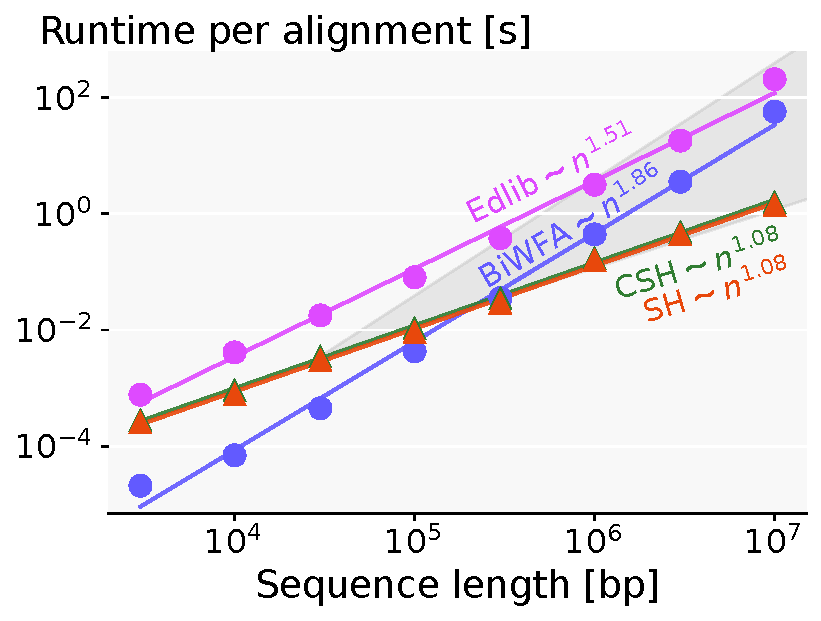
\includegraphics[width=0.4\linewidth]{imgs/fig4/tools_e0.01_labels.pdf}
  \label{GLOBALfig:scaling-n-1}}
  %\hfill
  \subfloat[$e{=}5\%$, exact matching]{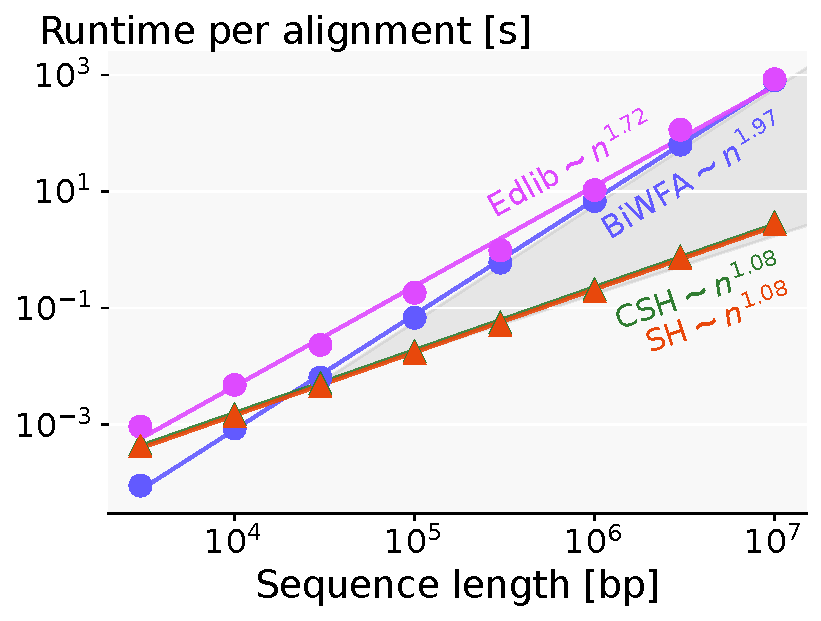
\includegraphics[width=0.4\linewidth]{imgs/fig4/tools_e0.05_labels.pdf}
  \label{GLOBALfig:scaling-n-5}}\\
  %\hfill
  \subfloat[$e{=}10\%$, inexact matching]{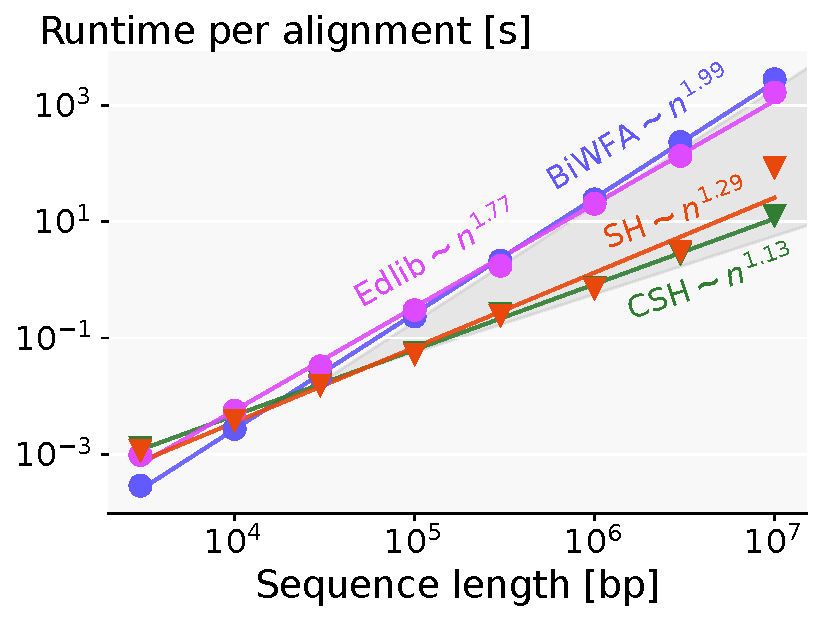
\includegraphics[width=0.4\linewidth]{imgs/fig4/tools_e0.1_labels.pdf}
  \label{GLOBALfig:scaling-n-10}}
  %\hfill
  \subfloat[$e{=}15\%$, inexact matching]{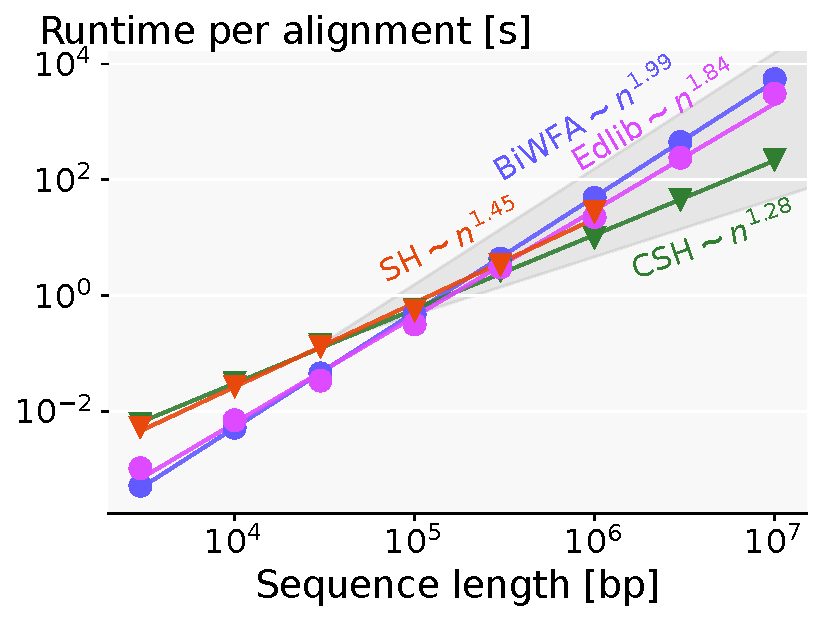
\includegraphics[width=0.4\linewidth]{imgs/fig4/tools_e0.15_labels.pdf}
  \label{GLOBALfig:scaling-n-15}}

  \caption[Runtime scaling with sequence length (multiple error rates)]{Log-log
    plots of the runtime for aligning \textbf{synthetic sequences} of increasing
    length for \astarpa \sh~(\SH), \astarpa \csh~(\CSH), \edlib~(\edlibsymbol)
    and \wfa~(\wfasymbol). The slopes of the bottom (top) of the dark-grey cones
    correspond to linear (quadratic) growth. For $e{\leq} 5\%$,
    \SH~(\shsymbolsq) and \CSH~(\cshsymbolsq) use $k{=}15$, $r{=}1$. For $e{\ge}
    10\%$, \SH~(\shsymbol) and \CSH~(\cshsymbol) use $k{=}15$, $r{=}2$. The
    missing data points for \SH at $e{=}15\%$ are due to exceeding the memory
    limit ($\qty{30}{GB}$). Each runtime is the average over $\lfloor 10^7 / n
    \rfloor$ alignments.}
  \label{GLOBALfig:scaling-n}
\end{figure}


\renewcommand\theenumi{\arabic{enumi}}
\renewcommand\labelenumi{{\rmfamily \arabic{enumi}.}}
\setlength{\leftmargini}{3mm}

%%%%%%%%%%%%%%%%%%%%%%%%%%%%%%%%%
%\section{Experimental Results}
\section{Evaluation} \label{TRIEsec:eval}
%%%%%%%%%%%%%%%%%%%%%%%%%%%%%%%%%

\begin{samepage}
In this section we present a thorough experimental
evaluation\footnote{\url{https://github.com/eth-sri/astarix/tree/RECOMB2020_experiments}}
of \astarix on simulated Illumina reads. Our evaluation demonstrates that:
\begin{enumerate}
  \item \astarix is faster than \dijkstra because the heuristic reduces the number of explored states by an order of magnitude.
  \item The runtime of \astarix scales better than state-of-the-art optimal
  aligners with increasing graph size, on a variety of reference graphs.
\end{enumerate}
\end{samepage}

\subsection{Implementation \astarix}

Our \astarix implementation uses an adjacency list graph data structure to
represent the reference and the trie in a unified way, representing each letter
by a separate edge object.
%\para{Reverse Complement Alignment}
To represent the reverse complementary walks in $\RG$, the vertices are doubled,
connected in the opposite direction, and labeled with complementary nucleotides
($\texttt{A} \leftrightarrow \texttt{T}$, $\texttt{C} \leftrightarrow
\texttt{G}$).
%
%\para{Default Parameters}
We do not limit the number of memoized heuristic function values
(\cref{TRIEpara:memoization}), but note we could do so by resetting the memoization
table periodically.
%
Our implementation of \dijkstra reuses the same \astarix codebase except the
use of a heuristic function (\ie, with $h \equiv 0$).
\subsection{Setting}
All evaluations were executed singled-threaded on an Intel Core i7-6700 CPU running
at 3.40GHz.

\para{Reference Graphs and Reads}
We designed three experiments utilizing three different reference graphs (in
\cref{TRIEtab:results}). The first is a linear graph without variation based on the
\textit{E.~coli} reference genome (strain: K-12 substr. MG1655,
ASM584v2~\cite{howe2019ensembl}). The other two are variation graphs taken from
the \pasgal evaluations~\cite{jain_accelerating_2019}: they are based on the
Leukocyte Receptor Complex (LRC, with \numprint{1099856} nodes and
\numprint{1144498} edges), and the Major Histocompatibility Complex (MHC1, with
\numprint{5138362} nodes and \numprint{5318019} edges).
%
We note that we do not evaluate on de Brujin graphs, since \pasgal does not
support cyclic graphs.

%\para{Reads}
For the \textit{E.~coli} dataset we used the ART tool~\cite{huang_art_2012} to simulate an
Illumina single-end read set with \numprint{10000} reads of length 100. For the LCR and
MHC1 datasets, we sampled \numprint{20000} single-end reads of length 100 from the already
generated sets in~\cite{jain_accelerating_2019} using the
Mason2~\cite{holtgrewe_mason_2010} simulator.

For \dijkstra and \astarix, the runtime complexity depends not only on the data
size, but also on the data content, including edit costs. More accurate
heuristics lead to better \A performance~\cite{pearl_discovery_1983}, which is
why we evaluate \astarix with costs corresponding more closely to Illumina error
profiles: $\Delta=(0,1,5,5)$.

\para{Metrics}
As all aligners evaluated in this work are provably optimal, we are mostly
interested in their performance.
%
To study the end-to-end performance of the optimal aligners, we use the
Snakemake~\cite{koster_snakemakescalable_2012} pipeline framework to measure the
execution time of every aligner (including the time spent on reading and
indexing the reference graph input and outputting the resulting alignments). We
note that the alignment phase dominates for all tools and experiments.

To judge the potential of heuristic functions, we measure not only the runtime
but also the number of states explored by \astarix and \dijkstra. This number
reflects the quality of the heuristic function rather than the speed of
computation of the heuristic, the implementation and the system parameters.
%"Fig. 3" (it also discusses explored states)}.
%The number of explored states is a more direct indicator for the algorithm's performance
%than the number of expanded states since the algorithm has to generate and consider
%all the neighbors of the states it expands.
%\todo{Harun: this argument only really works
%if computation of the heuristic is not a bottleneck. maybe make that more clear?}
%\subsection{Versions, commands, parameters for running all evaluated approaches}
In the following, we provide details on how we executed the compared tools.

\noindent
\begin{tabular}{lp{9.5cm}}
	\textbf{\pasgal} & \\
	\quad Obtained from & \url{https://github.com/ParBLiSS/PaSGAL} (Commit \texttt{50ad80c}) \\
	\quad Command & \texttt{PaSGAL -q reads.fq -r graph.vg -m vg -o output -t 1} \\
	\textbf{\bitparallel} & \\
	\quad Obtained from &
	\url{https://github.com/maickrau/GraphAligner/tree/WabiExperiments}
	(Commit \texttt{241565c}) \\
	\quad Command & \texttt{Aligner -f reads.fq -g graph.gfa >output} \\
	\textbf{\astarix} & \\
	\quad Obtained from & \astarixurlwithbranch \\
	\quad Command & \texttt{astarix align-optimal -f reads.fq -g graph.gfa >output} \\
	\textbf{\dijkstra} & \\
	\quad Obtained from & \astarixurlwithbranch \\
	\quad Command & \texttt{astarix align-optimal -f reads.fq -g graph.gfa -a dijkstra >output}
\end{tabular}
\subsection{Comparison of Optimal Aligners}

\para{Different Reference Graphs}
\cref{TRIEtab:results} shows the performance of optimal aligners across various
references. On all references, \astarix is consistently faster than \dijkstra,
which is consistently faster than \pasgal and \bitparallel. The memory usage of
\dijkstra is within a factor of 3 compared to \pasgal and \bitparallel. Due to
the heuristic memoization, the memory usage of \astarix can grow several times
compared to \dijkstra.

\begin{table}[H]
\centering
\ra{0.8}
\caption[Performance of optimal aligners for difference references]{Performance
of optimal aligners for different reference graphs.}\label{TRIEtab:results}
\sffamily
%\rowcolors{2}{gray!25}{white}

\renewrobustcmd{\bfseries}{\fontseries{b}\selectfont}
\renewrobustcmd{\boldmath}{}

\begin{tabular}{llrrrr}
\toprule
                && \multicolumn{4}{ c }{\textbf{Runtime} and \textbf{Memory}}\\
                \cmidrule{3-6}
\textbf{Genome graph} & \textbf{Size} & \bfseries \astarix & \dijkstra & \pasgal & \bitparallel\\
\midrule
    \rowcolor{gray!10}
    & &\bfseries \numprint{33} sec	 &\numprint{73} sec &\numprint{3272} sec &\numprint{4906} sec \\
    \rowcolor{gray!10}
    \multirow{-2}{*}{\textit{E. coli} (linear)} & \multirow{-2}{*}{4.7 Mbp} &\numprint{0.66} GB   &\numprint{0.66} GB &\numprint{0.55} GB   &\numprint{0.43} GB \\
    & &\bfseries \numprint{437} sec &\numprint{940} sec	 &\numprint{1614} sec & \\
    \multirow{-2}{*}{LCR (graph)} & \multirow{-2}{*}{1 Mbp} &\numprint{1.12} GB   &\numprint{1.09} GB &\numprint{0.30} GB   & \multirow{-2}{*}{SegFault}\\
    \rowcolor{gray!10}
    & &\bfseries \numprint{1282} sec &\numprint{1588} sec & >\numprint{7200} sec &\\
    \rowcolor{gray!10}
    \multirow{-2}{*}{MHC1 (graph)} & \multirow{-2}{*}{5 Mbp} &\numprint{4.35} GB   &\numprint{1.21} GB    &  \numprint{0.87} GB         		&\multirow{-2}{*}{SegFault}\\
\bottomrule
\end{tabular}

\end{table}

\para{Scaling with Reference Graph Size}
\cref{TRIEfig:scaling_with_graphsize} compares the performance of existing optimal
aligners. \bitparallel and \pasgal always explore all states, thus their
average-case reaches the worst-case complexity of $\Oh(\lvert \AG \rvert) =
\Oh(m \concat \RG)$. Due to the trie indexing, the runtime of \astarix and
\dijkstra scales in the reference size with a polynomial of power around $0.2$
versus the expected linear dependency of \bitparallel and \pasgal.

The heuristic function of \astarix demonstrates a 2-fold speed-up over
\dijkstra. This is possible due to the highly branching trie structure, which
allows skipping the explicit exploration for the majority of starting nodes. 

\begin{figure}[t]
  \begin{subfigure}{.49\textwidth}
    \centering
    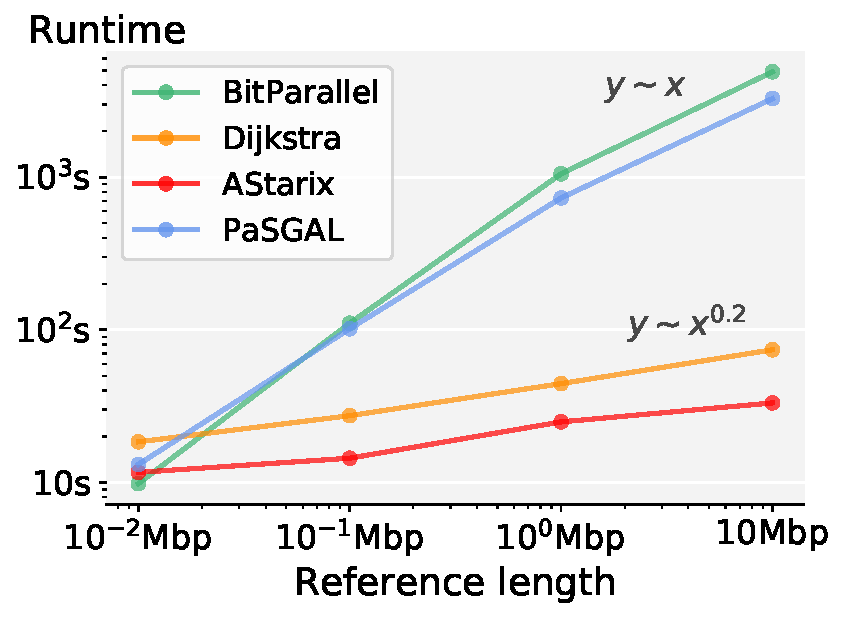
\includegraphics[width=\linewidth]{\dir/figs/cmp/performance_vs_genomesize-head_Mbpxs.pdf}
  \end{subfigure}
  \begin{subfigure}{.49\textwidth}
    \centering
    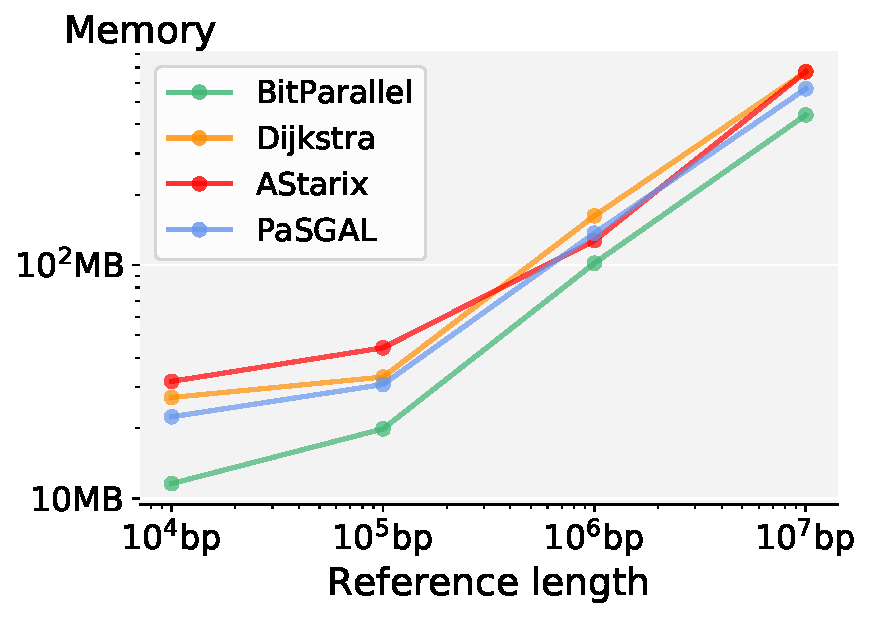
\includegraphics[width=\linewidth]{\dir/figs/cmp/memory_vs_genomesize-headxmax_rss.pdf}
  \end{subfigure}
  \caption{Comparison of overall runtime and memory usage of optimal aligners
     with increasing prefixes of E. coli as references.}
  \label{TRIEfig:scaling_with_graphsize}
\end{figure}

\subsection{\A scaling and speedup}
To measure the speedup caused by the heuristic function, we compare the number
of not only the expanded, but also of explored states (the latter number is
never smaller, see~\cref{TRIEsubsec:general-astar} and the example
in~\cref{TRIEfig:heuristic-benefit}) between \astarix and \dijkstra on the MHC1
dataset.

\cref{TRIEfig:scaling_with_errors} demonstrates the benefit of the heuristic
function in terms of both alignment time and number of explored states. Most
importantly, \astarix scales much better with increasing number of errors in the
read, compared to \dijkstra. More specifically, the number of states explored by
\dijkstra, as a function of alignment cost, grows exponentially with a base of 
around 10, whereas the base for \astarix is around 3 (the empirical complexity is
estimated as a best exponential fit \mbox{$\mli{exploredStates} \sim a \cdot
\mli{score}^b$}).

The horizontal black line in \cref{TRIEfig:scaling_with_errors} denotes the total
number of states $\lvert \RG \rvert \cdot \lvert q \rvert$, which is always
explored by \bitparallel and \pasgal. On the other hand, any aligner must
explore at least $m = \lvert q \rvert$ states, which we show as a horizontal
dashed line. This lower bound is determined by the fact that at least the states
on a best alignment need to be explored.

\begin{figure}[t]
  \begin{subfigure}{.45\textwidth}
    \centering
    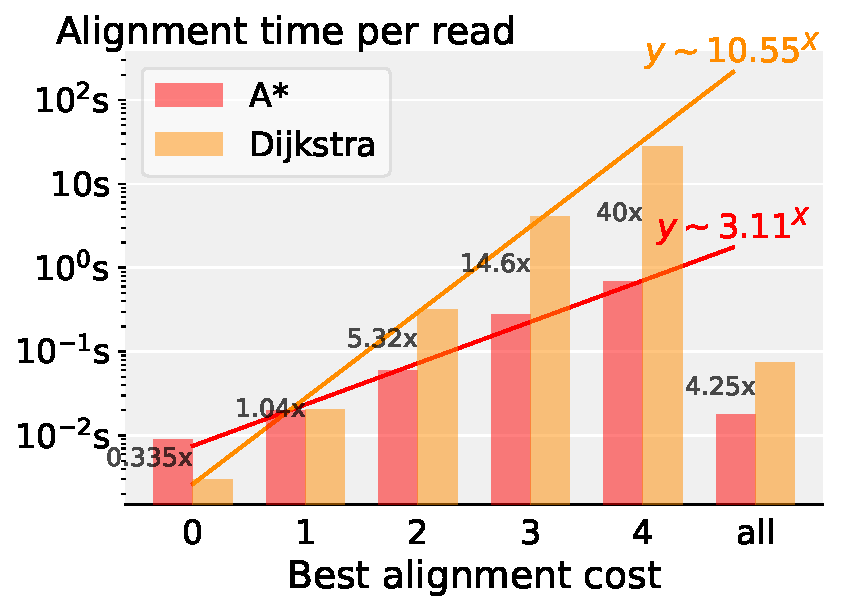
\includegraphics[width=\linewidth]{figs/cmp/heuristic_MHC1_cost-t(map).pdf}
  \end{subfigure}%~\hspace{1em}
  \begin{subfigure}{.45\textwidth}
    \centering
    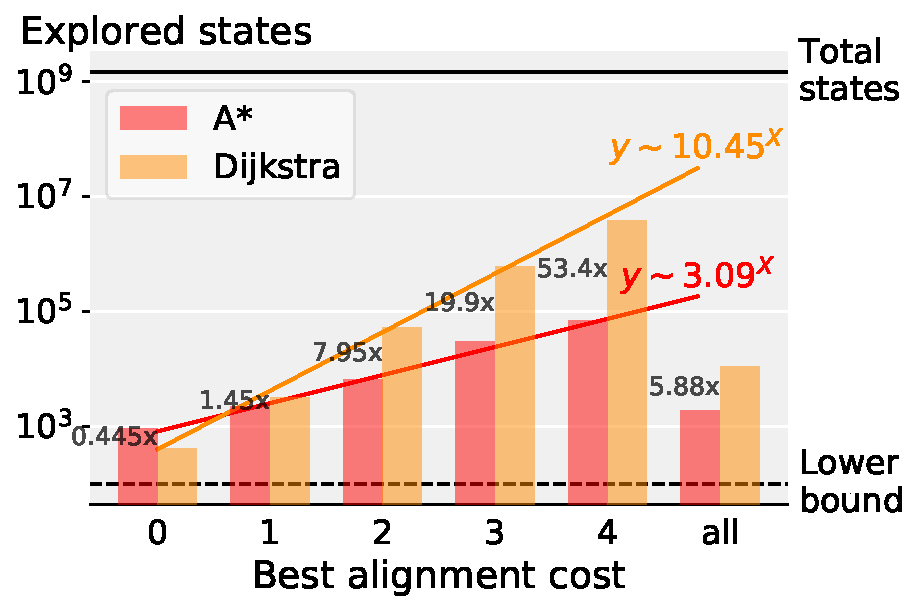
\includegraphics[width=\linewidth]{figs/cmp/heuristic_MHC1_cost-explored_states.pdf}
  \end{subfigure}%
  \caption[Performance scaling with alignment cost]{Comparison of \A and \dijkstra in terms of mean alignment runtime per read and mean explored states depending on the alignment cost on MHC1.}
  \label{TRIEfig:scaling_with_errors}
\end{figure}
